\documentclass[a4paper,10pt]{book}
\usepackage[utf8x]{inputenc}
\usepackage[italian]{babel}
\usepackage{graphicx}
%\usepackage{titlesec}
\usepackage{eurosym}

\title{La scoperta dei Ceccagno in Brasile}
\author{Rolando Ceccagno}
%\date{December 12, 2007}

\begin{document}

\maketitle
\tableofcontents
%\listoffigures

\chapter*{Premessa}

Questo diario non ha nessuna pretesa letteraria. E’stato scritto, a braccio, alla fine di ogni giornata, pertanto conterrà delle imprecisioni inerenti a persone, nomi di cose e luoghi; inoltre sarà zeppo di strafalcioni grammaticali. Ho studiato agraria, in collegio a Padova. Poi, a Milano, ho frequentato l’Istituto Tecnico Serale "E. Conti" dal 1943 al 1947. Immaginatevi in che tempi.

Un diario è anche un colloquio con se stessi, con piccole riflessioni, ovvie considerazioni e, magari, pieno di banalità.

Per la posizione genealogica delle persone che verranno menzionate, sarà utile consultare gli alberi genealogici, ancora incompleti, dei Ceccagnos do Brasil di \textbf{Felice} e di quelli italiani di \textbf{Filippo}.

Ipotizzo che Felice (1847) e Filippo (1857) potrebbero essere, a mio giudizio, cugini.

\begin{figure}[htp]
\centering
\includegraphics[width=0.9\textwidth]{../img/01-nonno-filippo.png}\label{fig:01-nonno-filippo}
\caption{\textbf{1931 Galzignano Terme (PD) Nonno Filippo Ceccagno i suoi nipoti}\newline Da sinistra, dietro in piedi: ?, \textbf{Itala}, zia Maria, \textbf{Carmen}, zio Dario, Livio, maestra Romagnoli, \textbf{Nonno Filippo}\newline Davanti Dorina, Idalga, Flora con Tiberio, Sergio, ?, zia Adelaide con \textbf{Nereo}, ? con ?, madre maestra Romagnoli con \textbf{Rolando}, Carla e Tersilla} 
\end{figure}

\begin{figure}[htp]
\centering
\includegraphics[width=0.9\textwidth]{../img/02-ceccagno-brasile.png}\label{fig:02-ceccagno-brasile}
\caption{\textbf{1911 A Protasio Alves, Rio Grande do Sul}\newline Da sinistra, Francesco*, Stella* Sanavio Ceccagno, \textbf{Felice* Ceccagno}, Giosuè* con Angelo, Marietta Maschio con Joáo, Alessandro* con Pedro Antonio, Giuseppina Bolzan con Felix\newline * Da Abano Terme(PD), sbarcati nel porto di Rio Grande nel febbraio del 1891}
\end{figure}

% \begin{table}[htp]
% \centering
% \begin{tabular}{ c c }
%   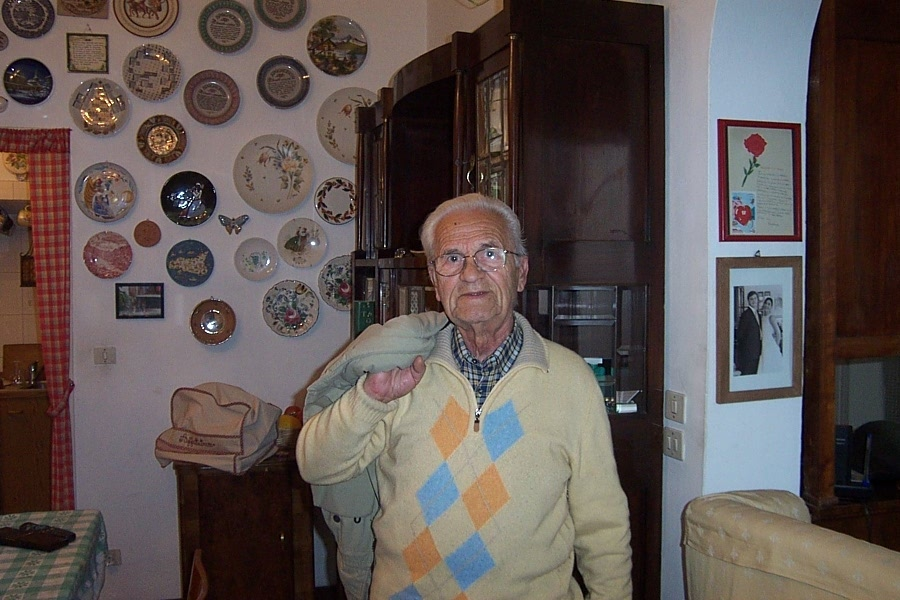
\includegraphics[height=0.5\textwidth]{../img/03-rolando.png}\label{fig:03-rolando}
%   &
%   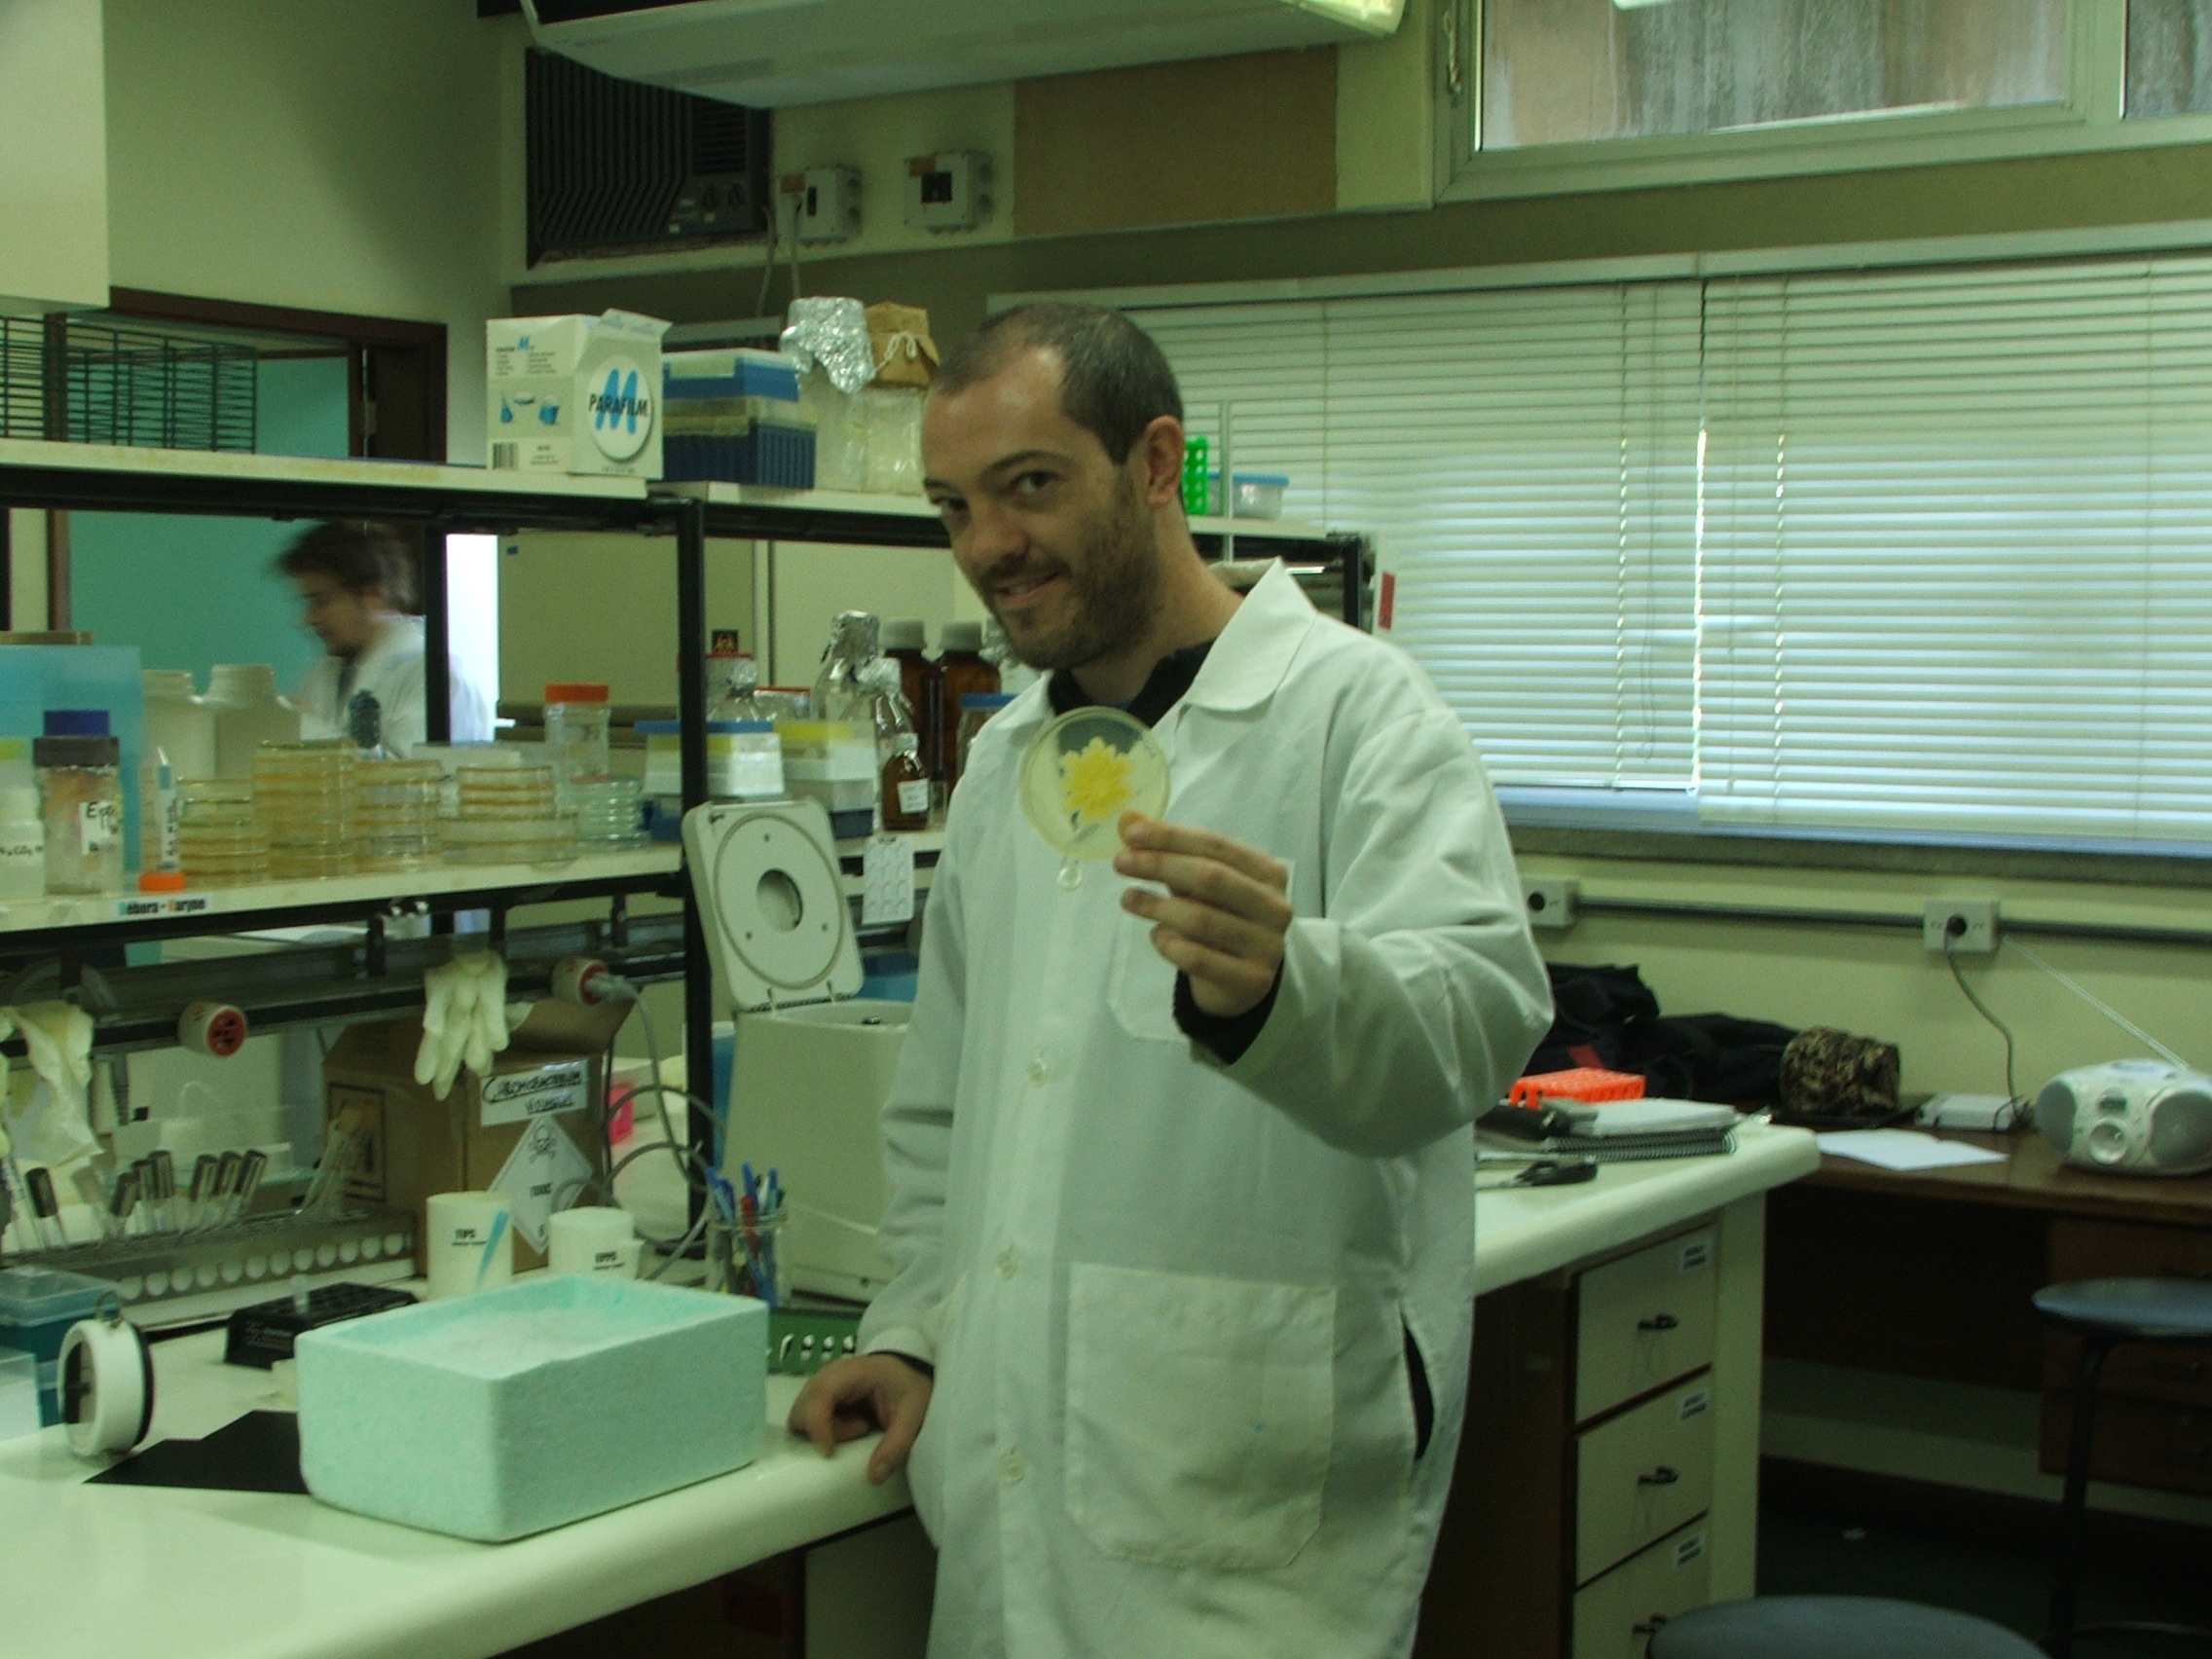
\includegraphics[height=0.5\textwidth]{../img/04-ricardo.png}\label{fig:04-ricardo}\\
% 
% %  \caption{\textbf{Rolando Ceccagno} - 1927 Galzignano Terme (PD) \textbf{Italia}}
% %  &
% %  \caption{\textbf{Ricardo Cecagno} - 1980 Paraí - Rio Grande do Sul - \textbf{Brasil}}
% \end{tabular}
% \end{table}

\begin{figure}[htp]
\centering
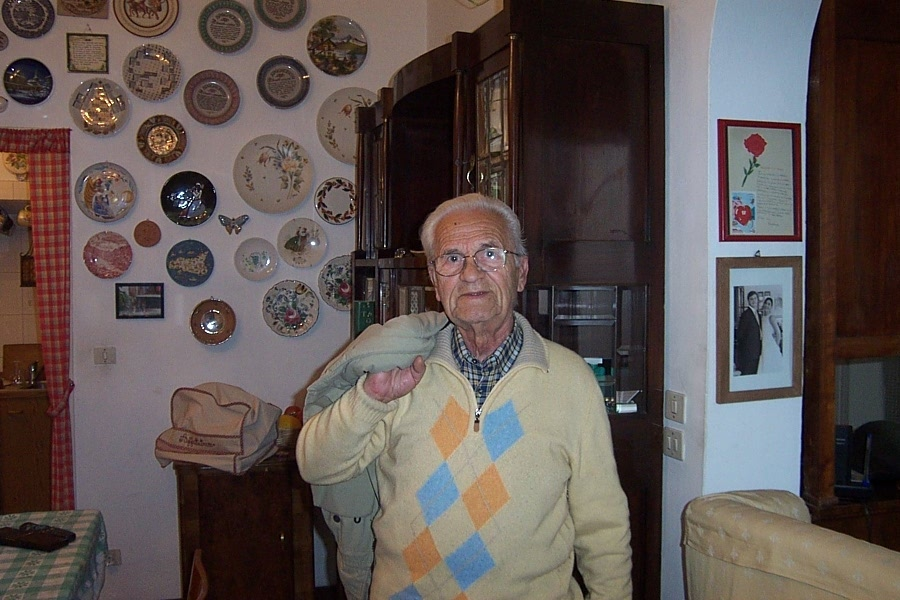
\includegraphics[width=0.5\textwidth]{../img/03-rolando.png}\label{fig:03-rolando.png}
\caption{\textbf{Rolando Ceccagno} - 1927 Galzignano Terme (PD) \textbf{Italia}}
\end{figure}

\begin{figure}[htp]
\centering
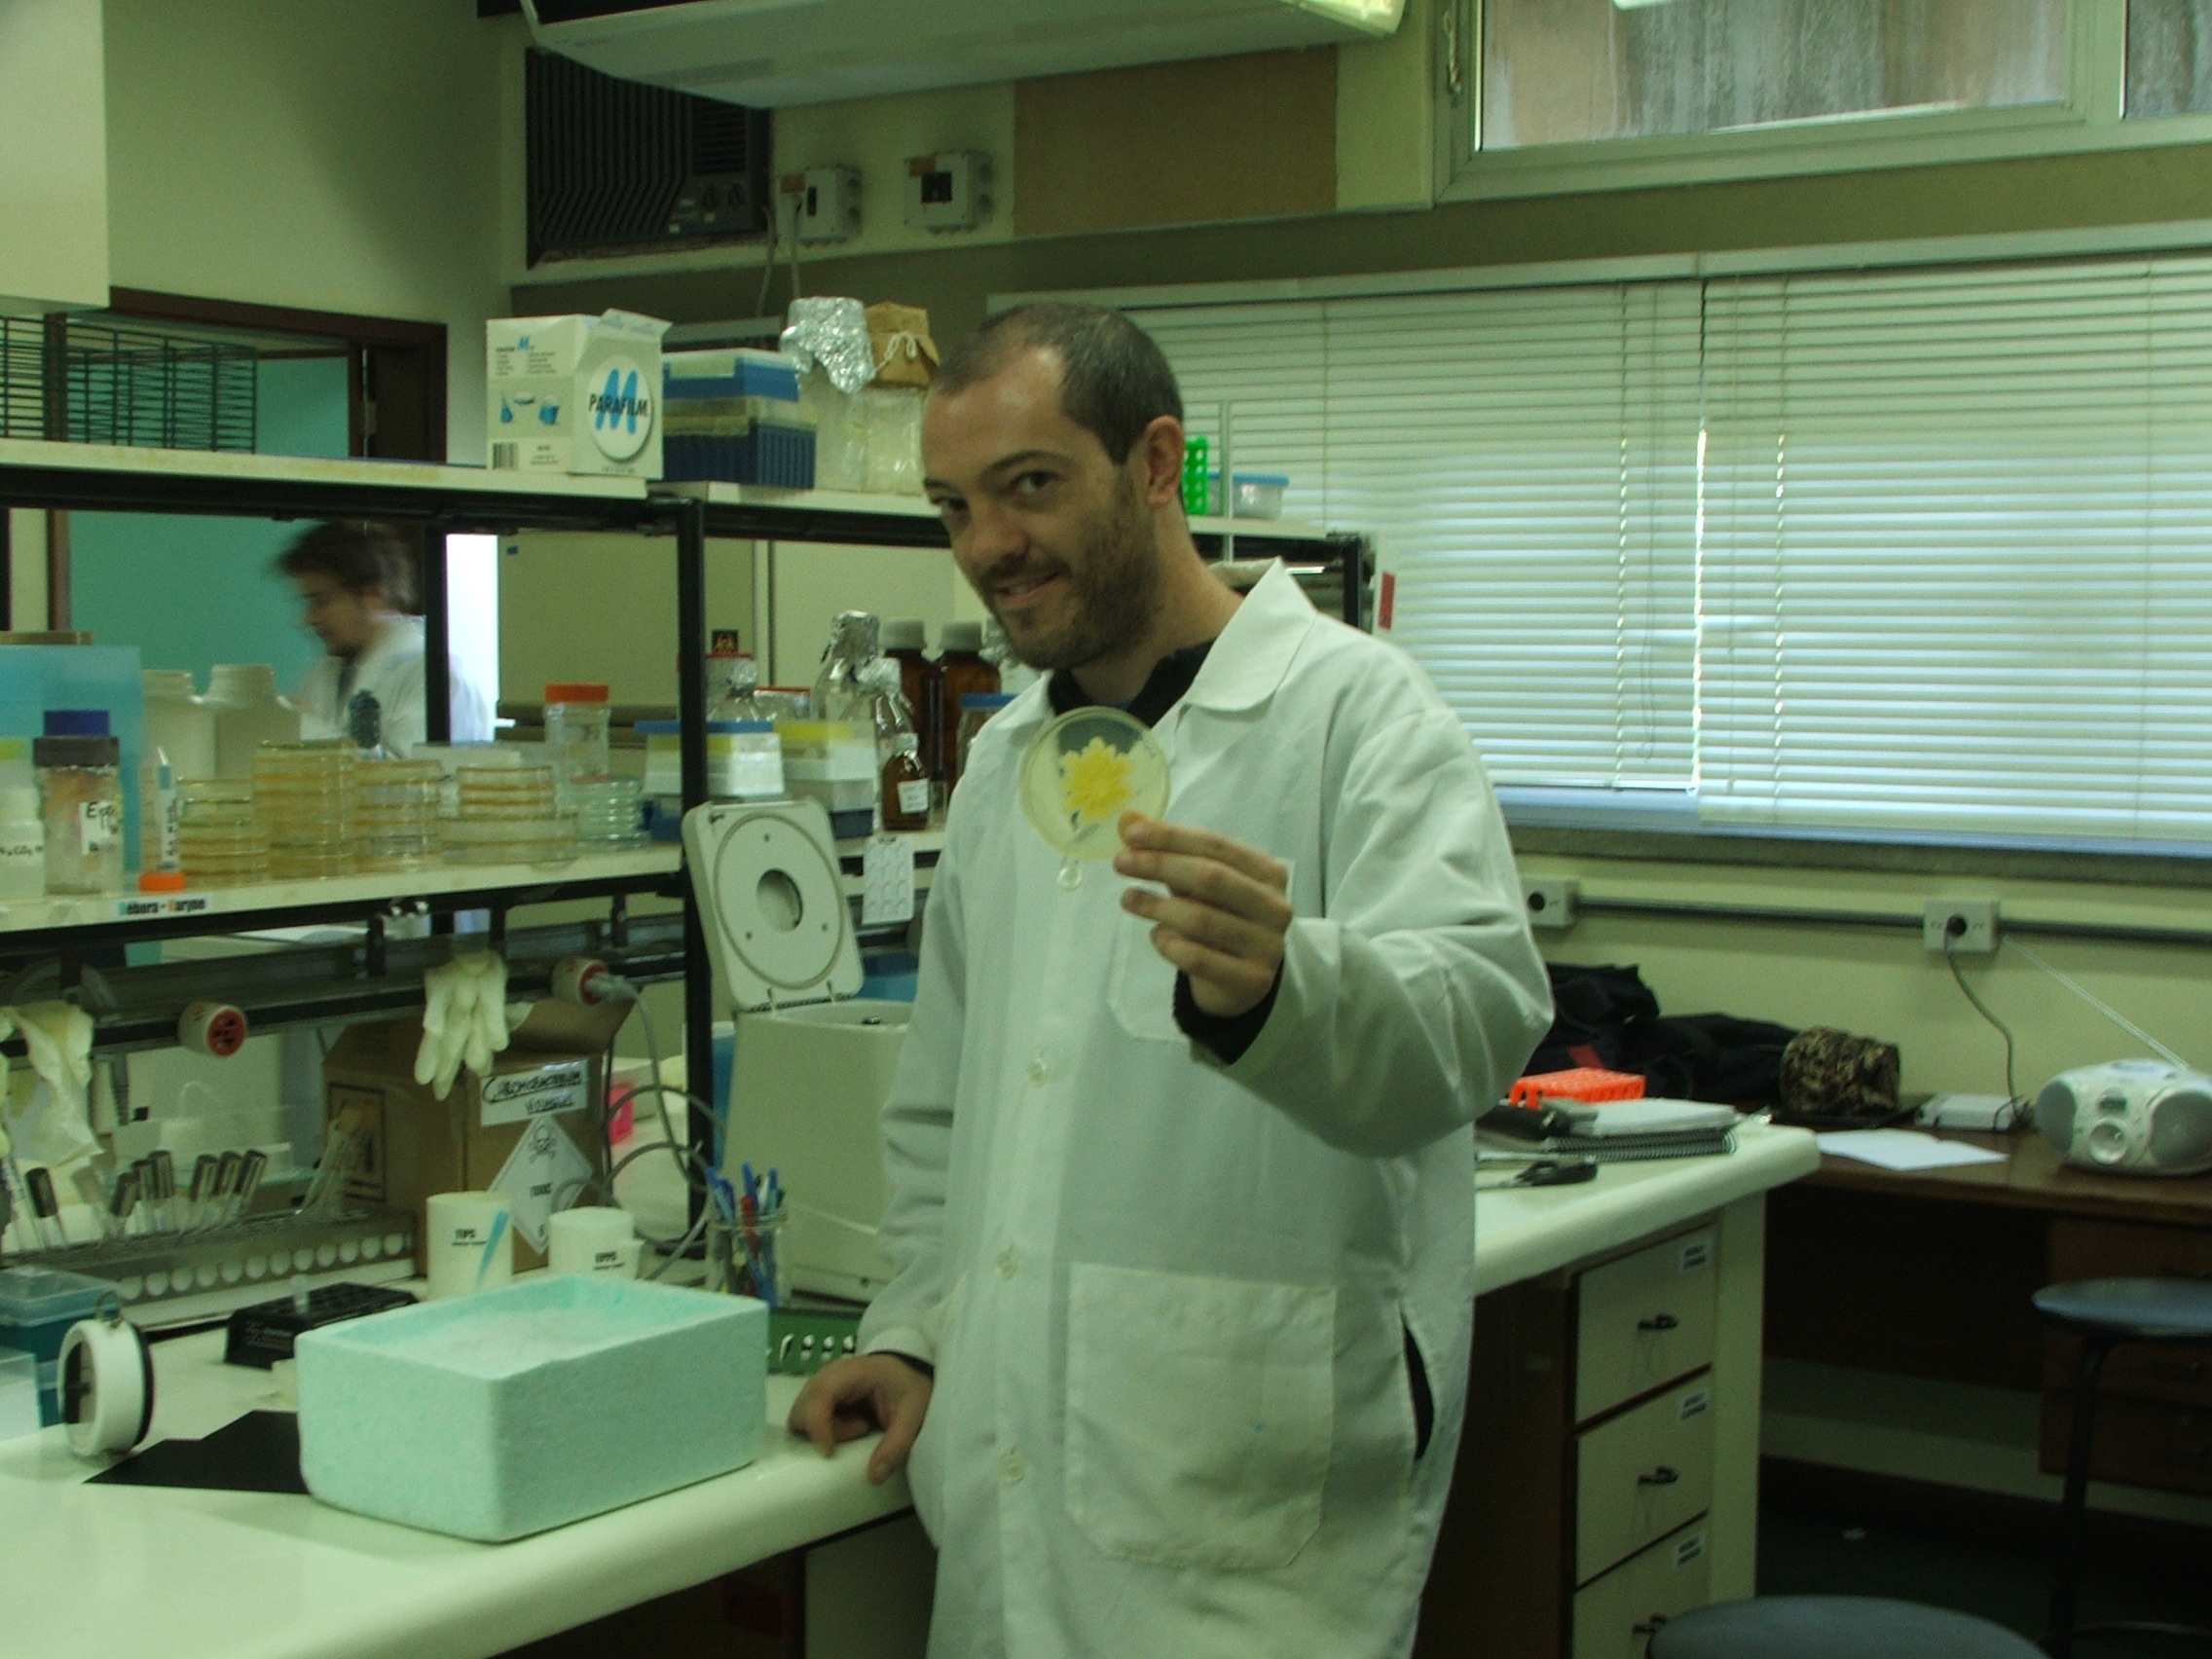
\includegraphics[width=0.5\textwidth]{../img/04-ricardo.png}\label{fig:04-ricardo.png}
\caption{\textbf{Ricardo Cecagno} - 1980 Paraí - Rio Grande do Sul - \textbf{Brasil}}
\end{figure}

\begin{tabular}{ c c }
  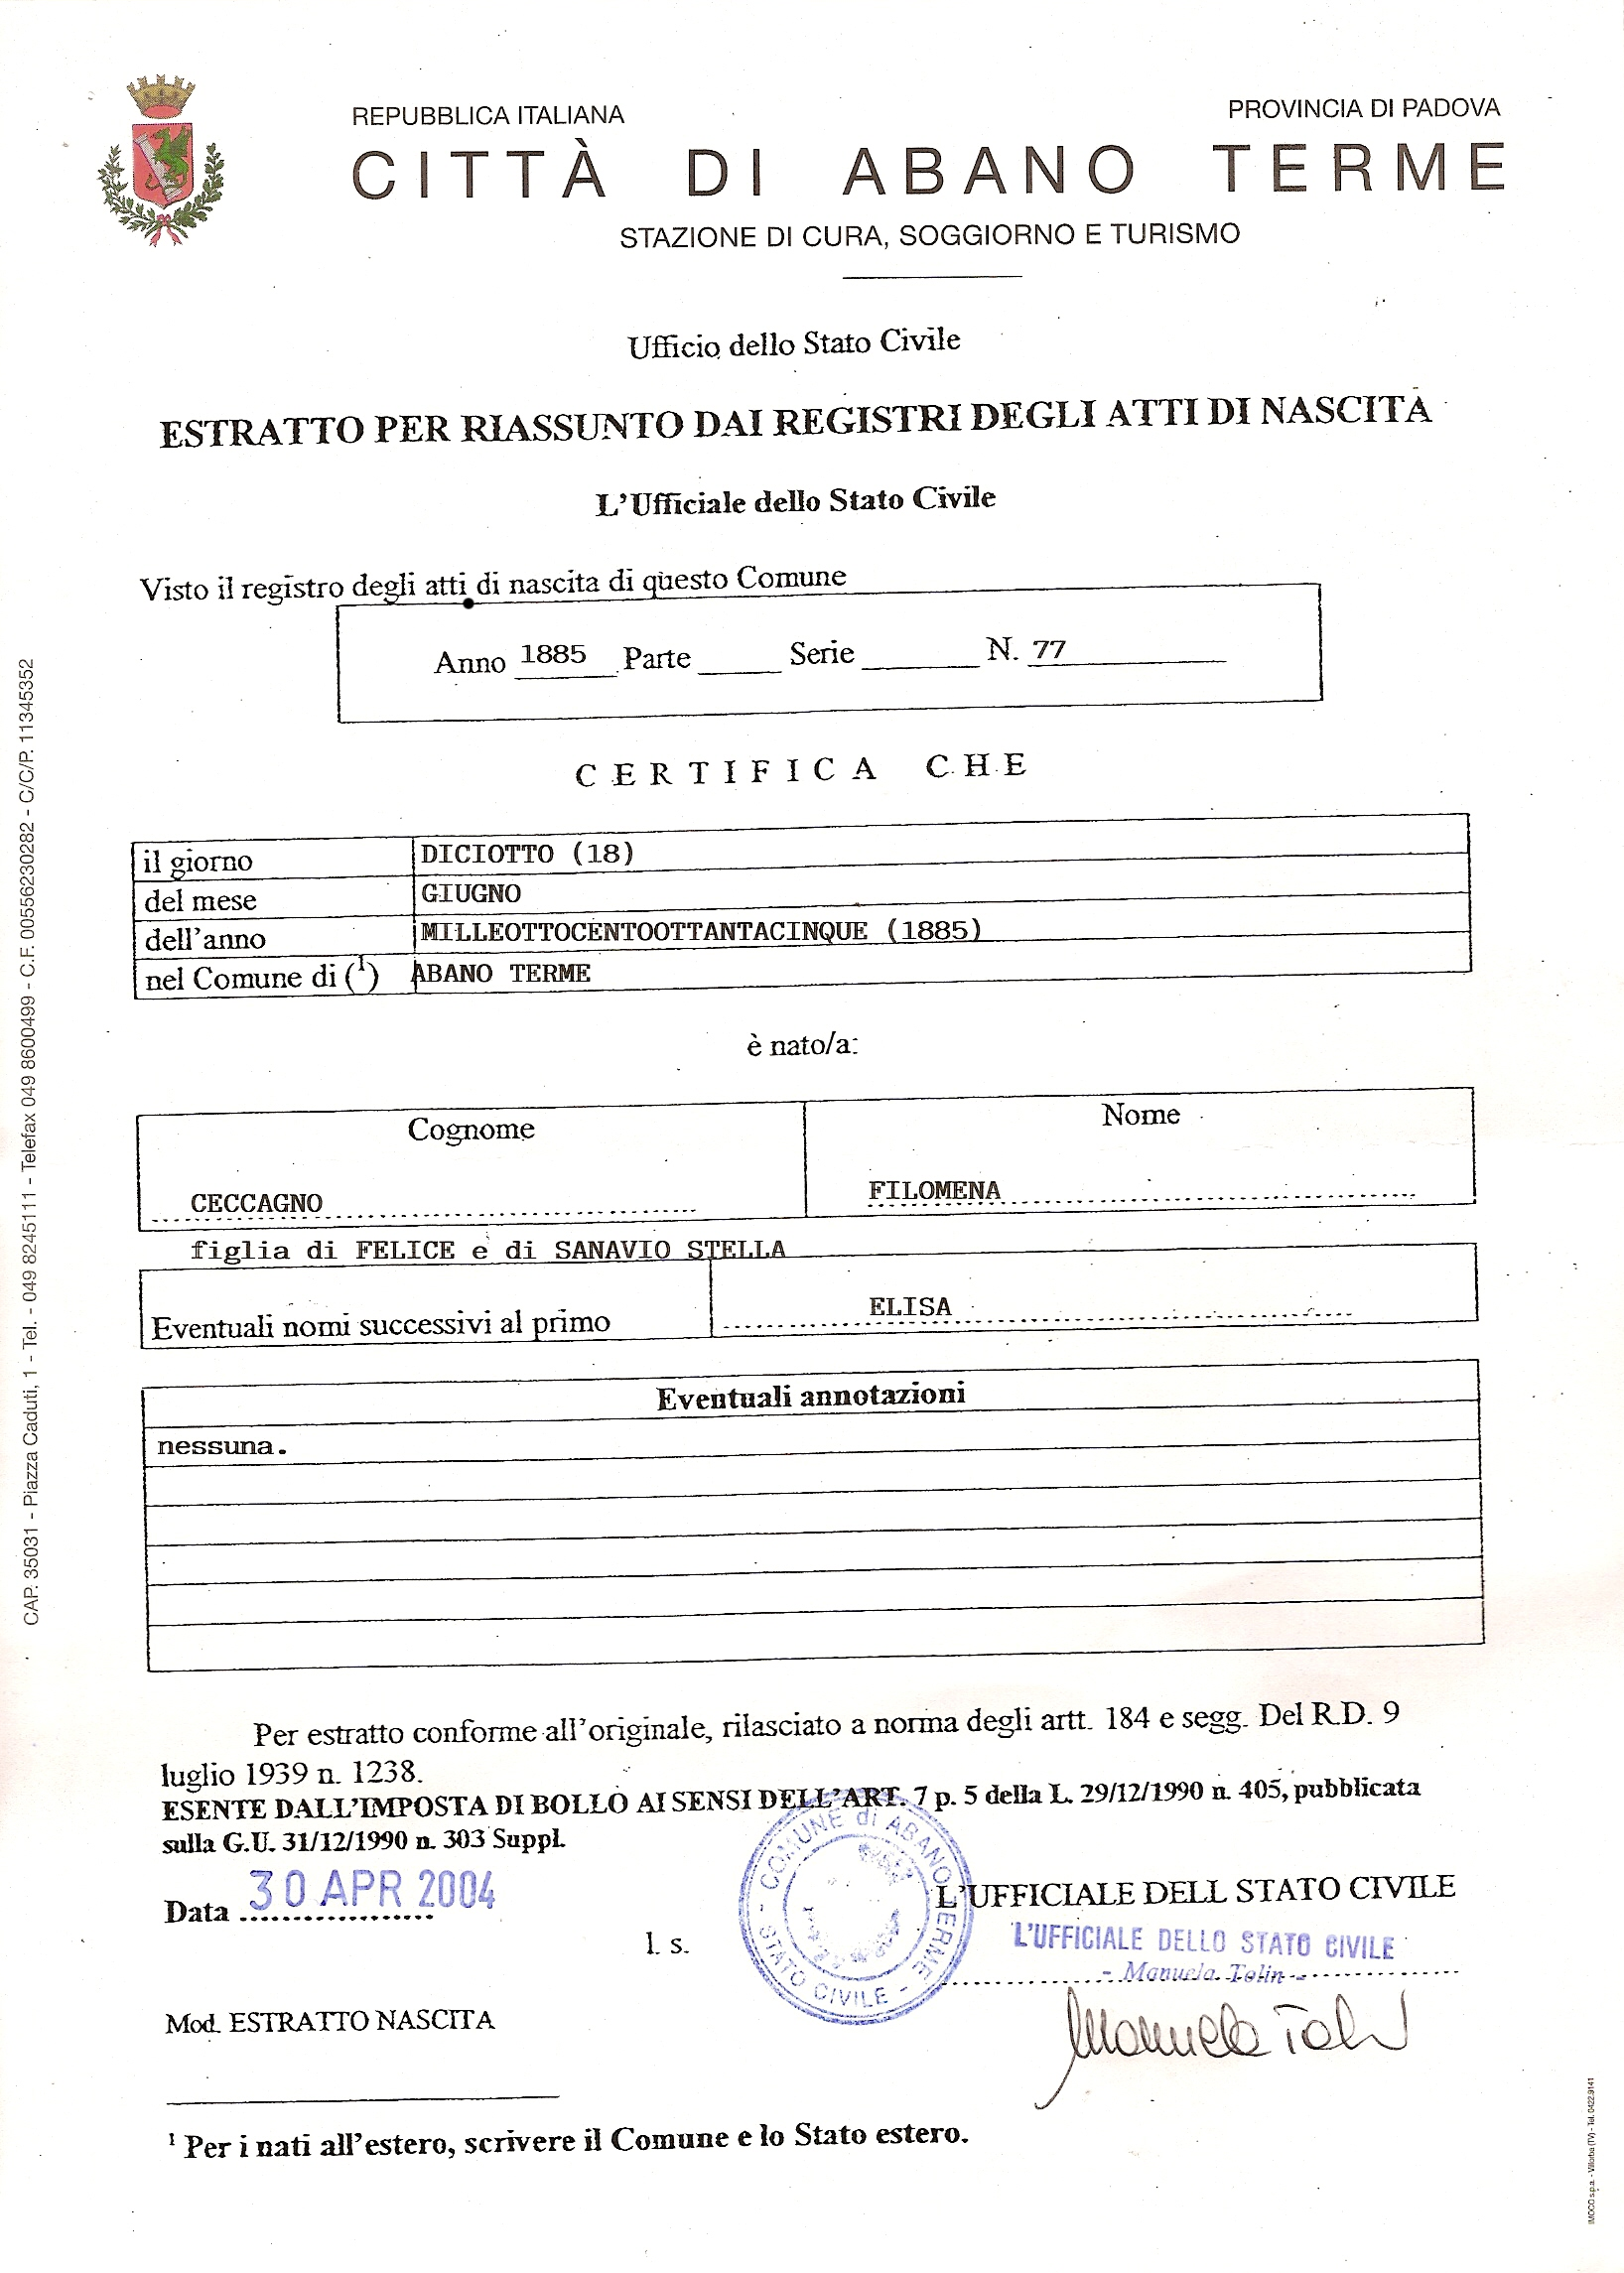
\includegraphics[height=0.35\textheight]{../img/05-filomena.png}\label{fig:05-filomena}
  & 
  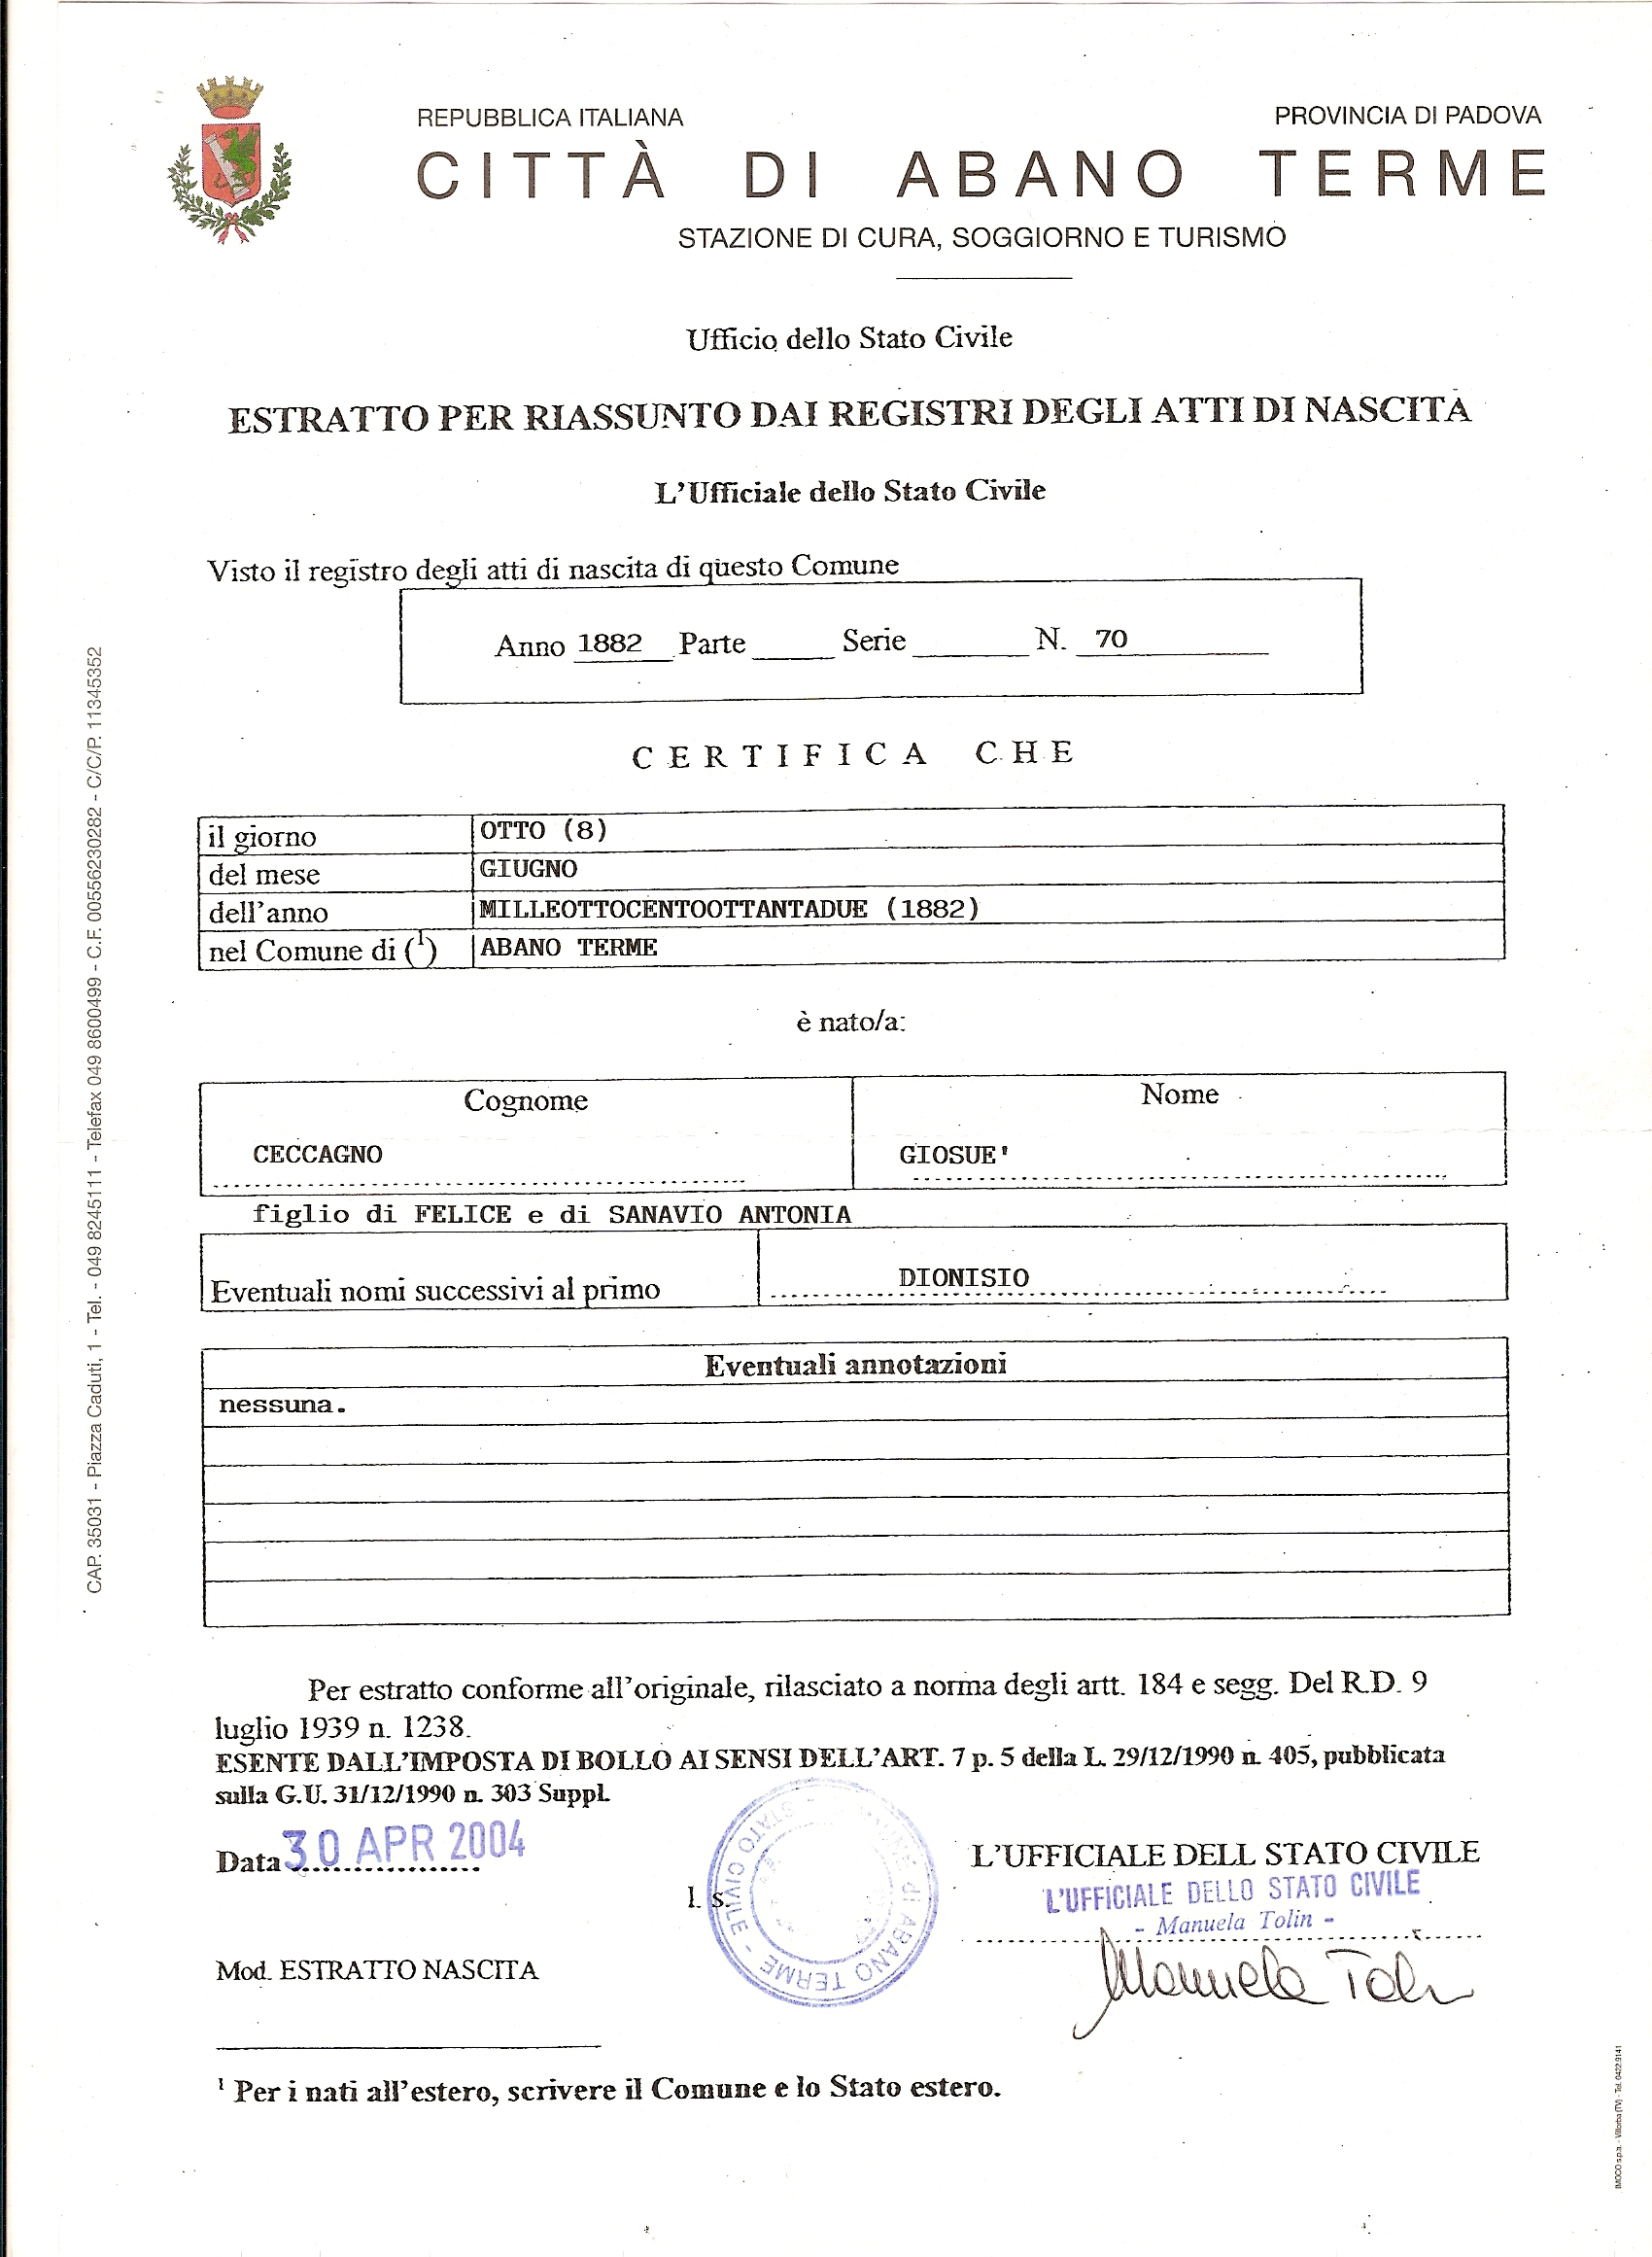
\includegraphics[height=0.35\textheight]{../img/06-giosue.png}\label{fig:06-giosue}
  \\ \\
  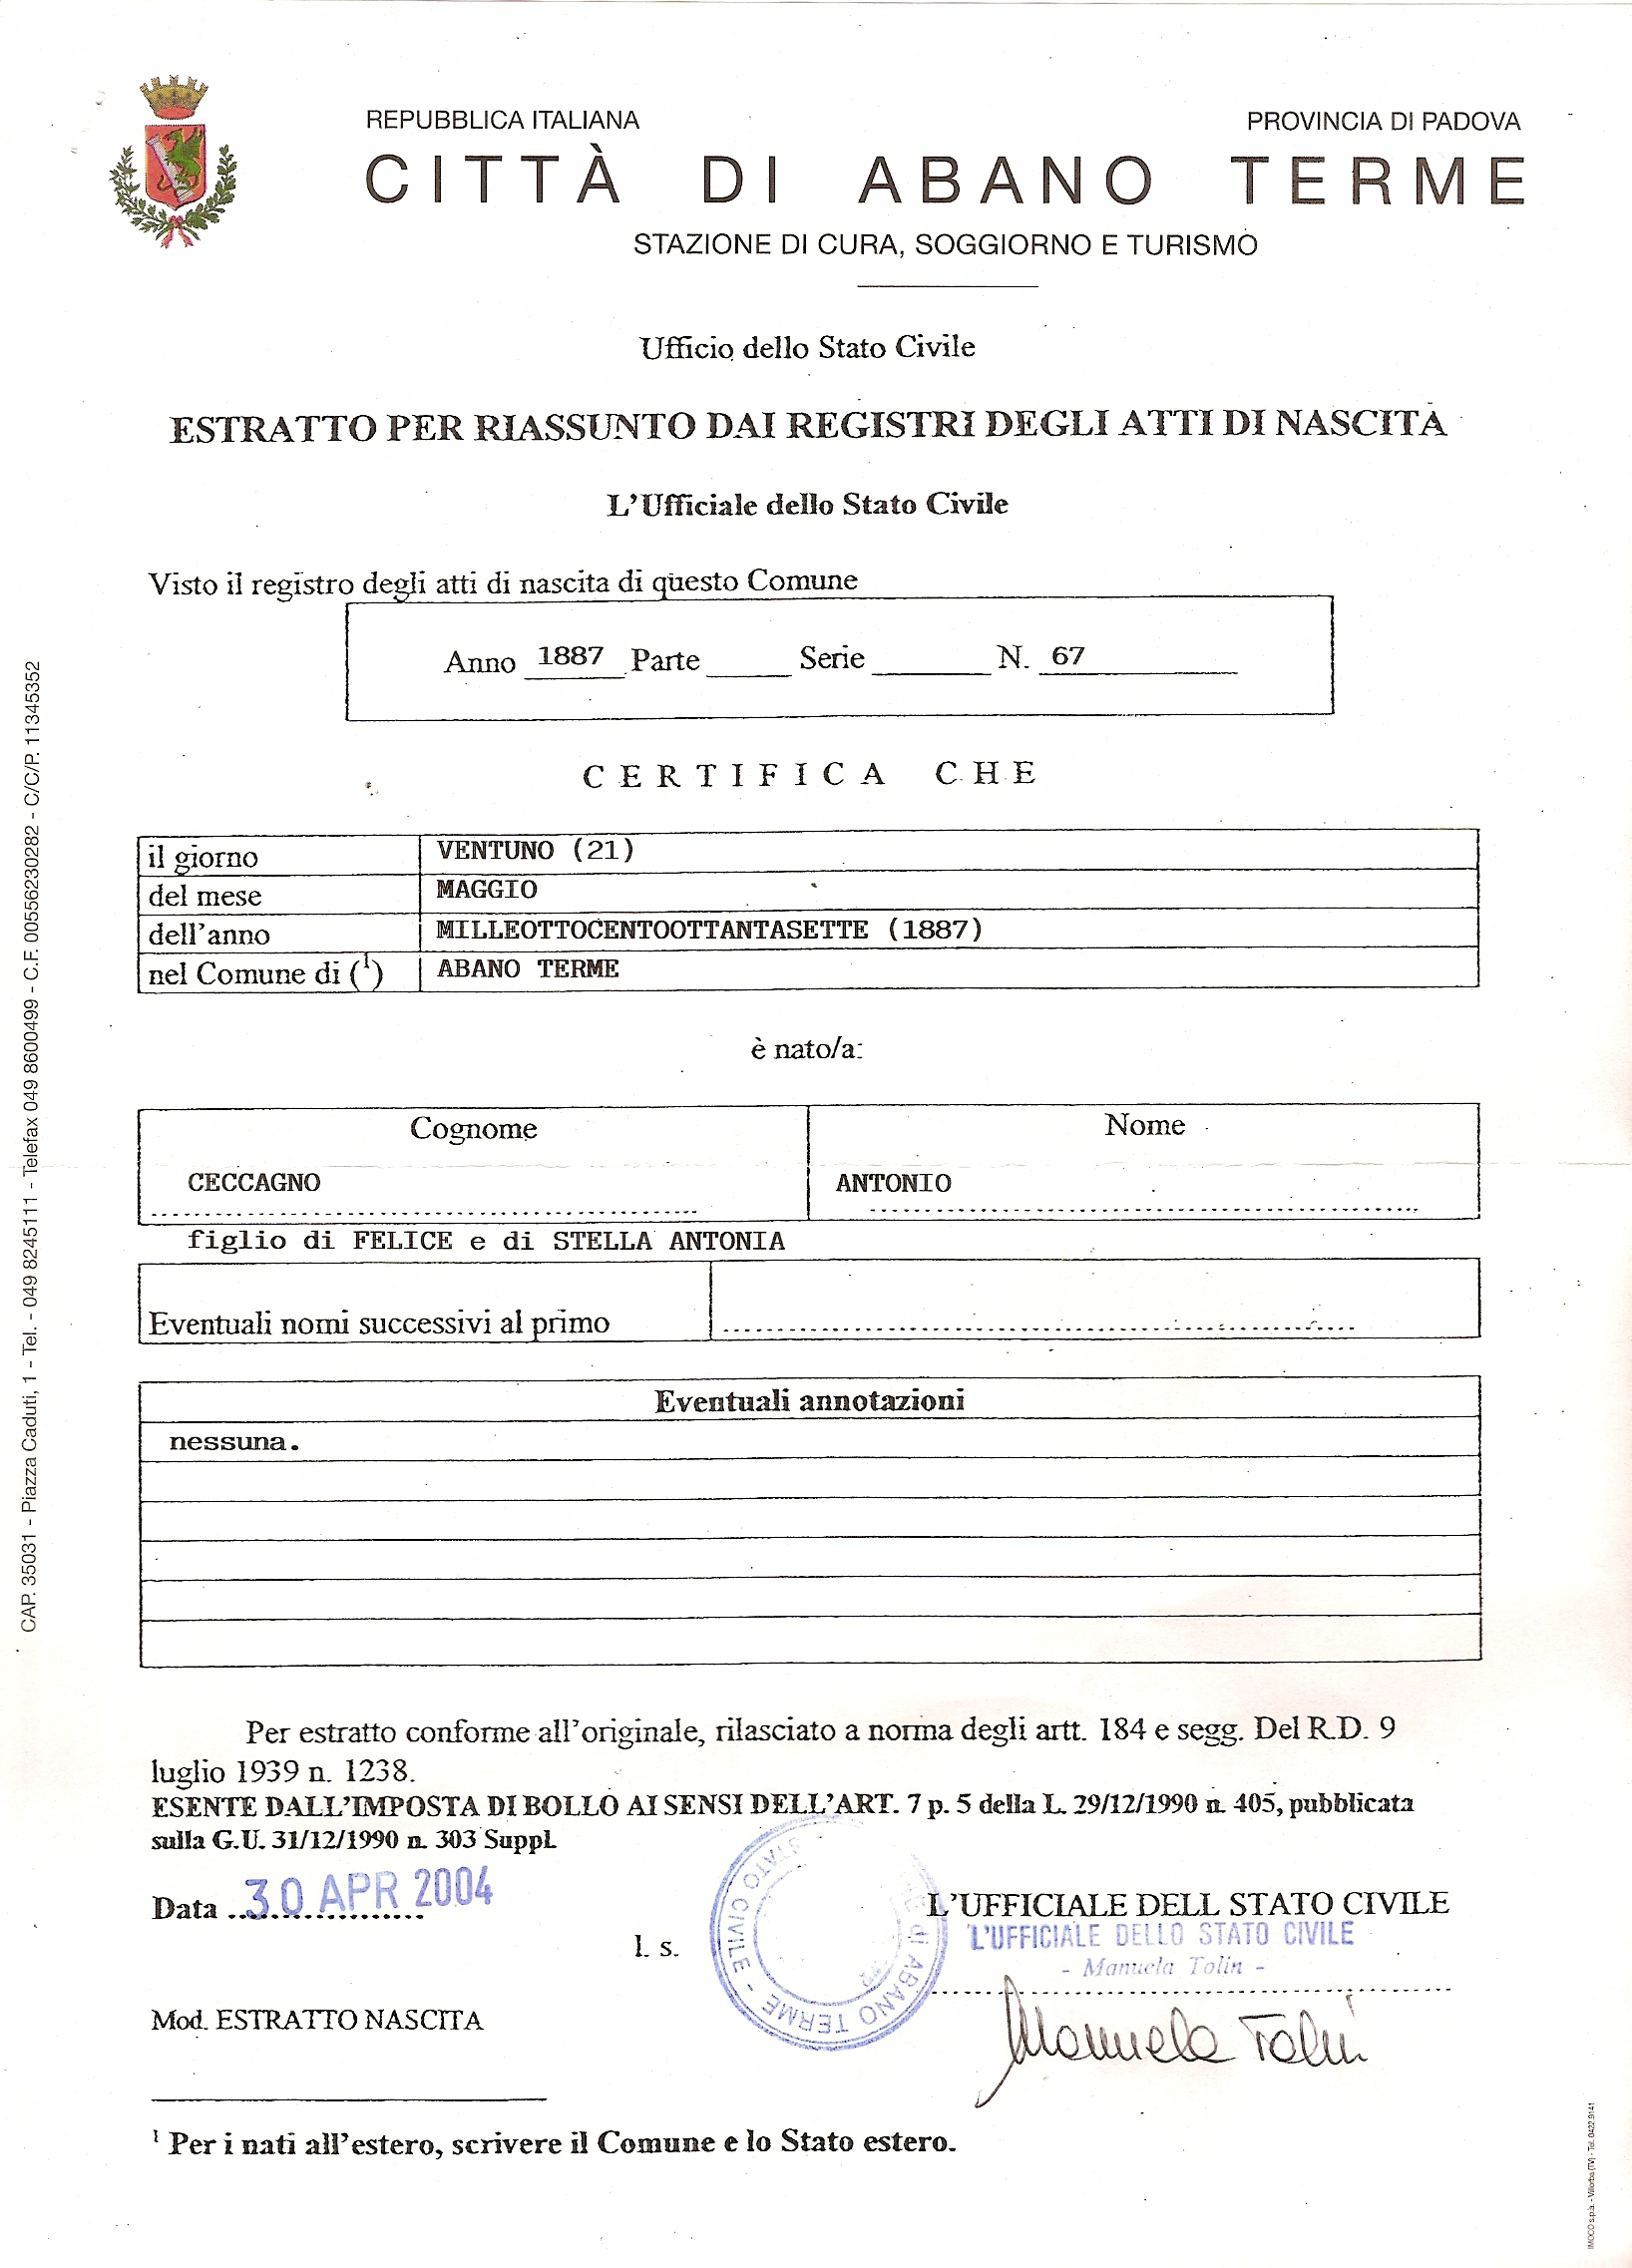
\includegraphics[height=0.35\textheight]{../img/07-antonio.png}\label{fig:07-antonio}
  &
  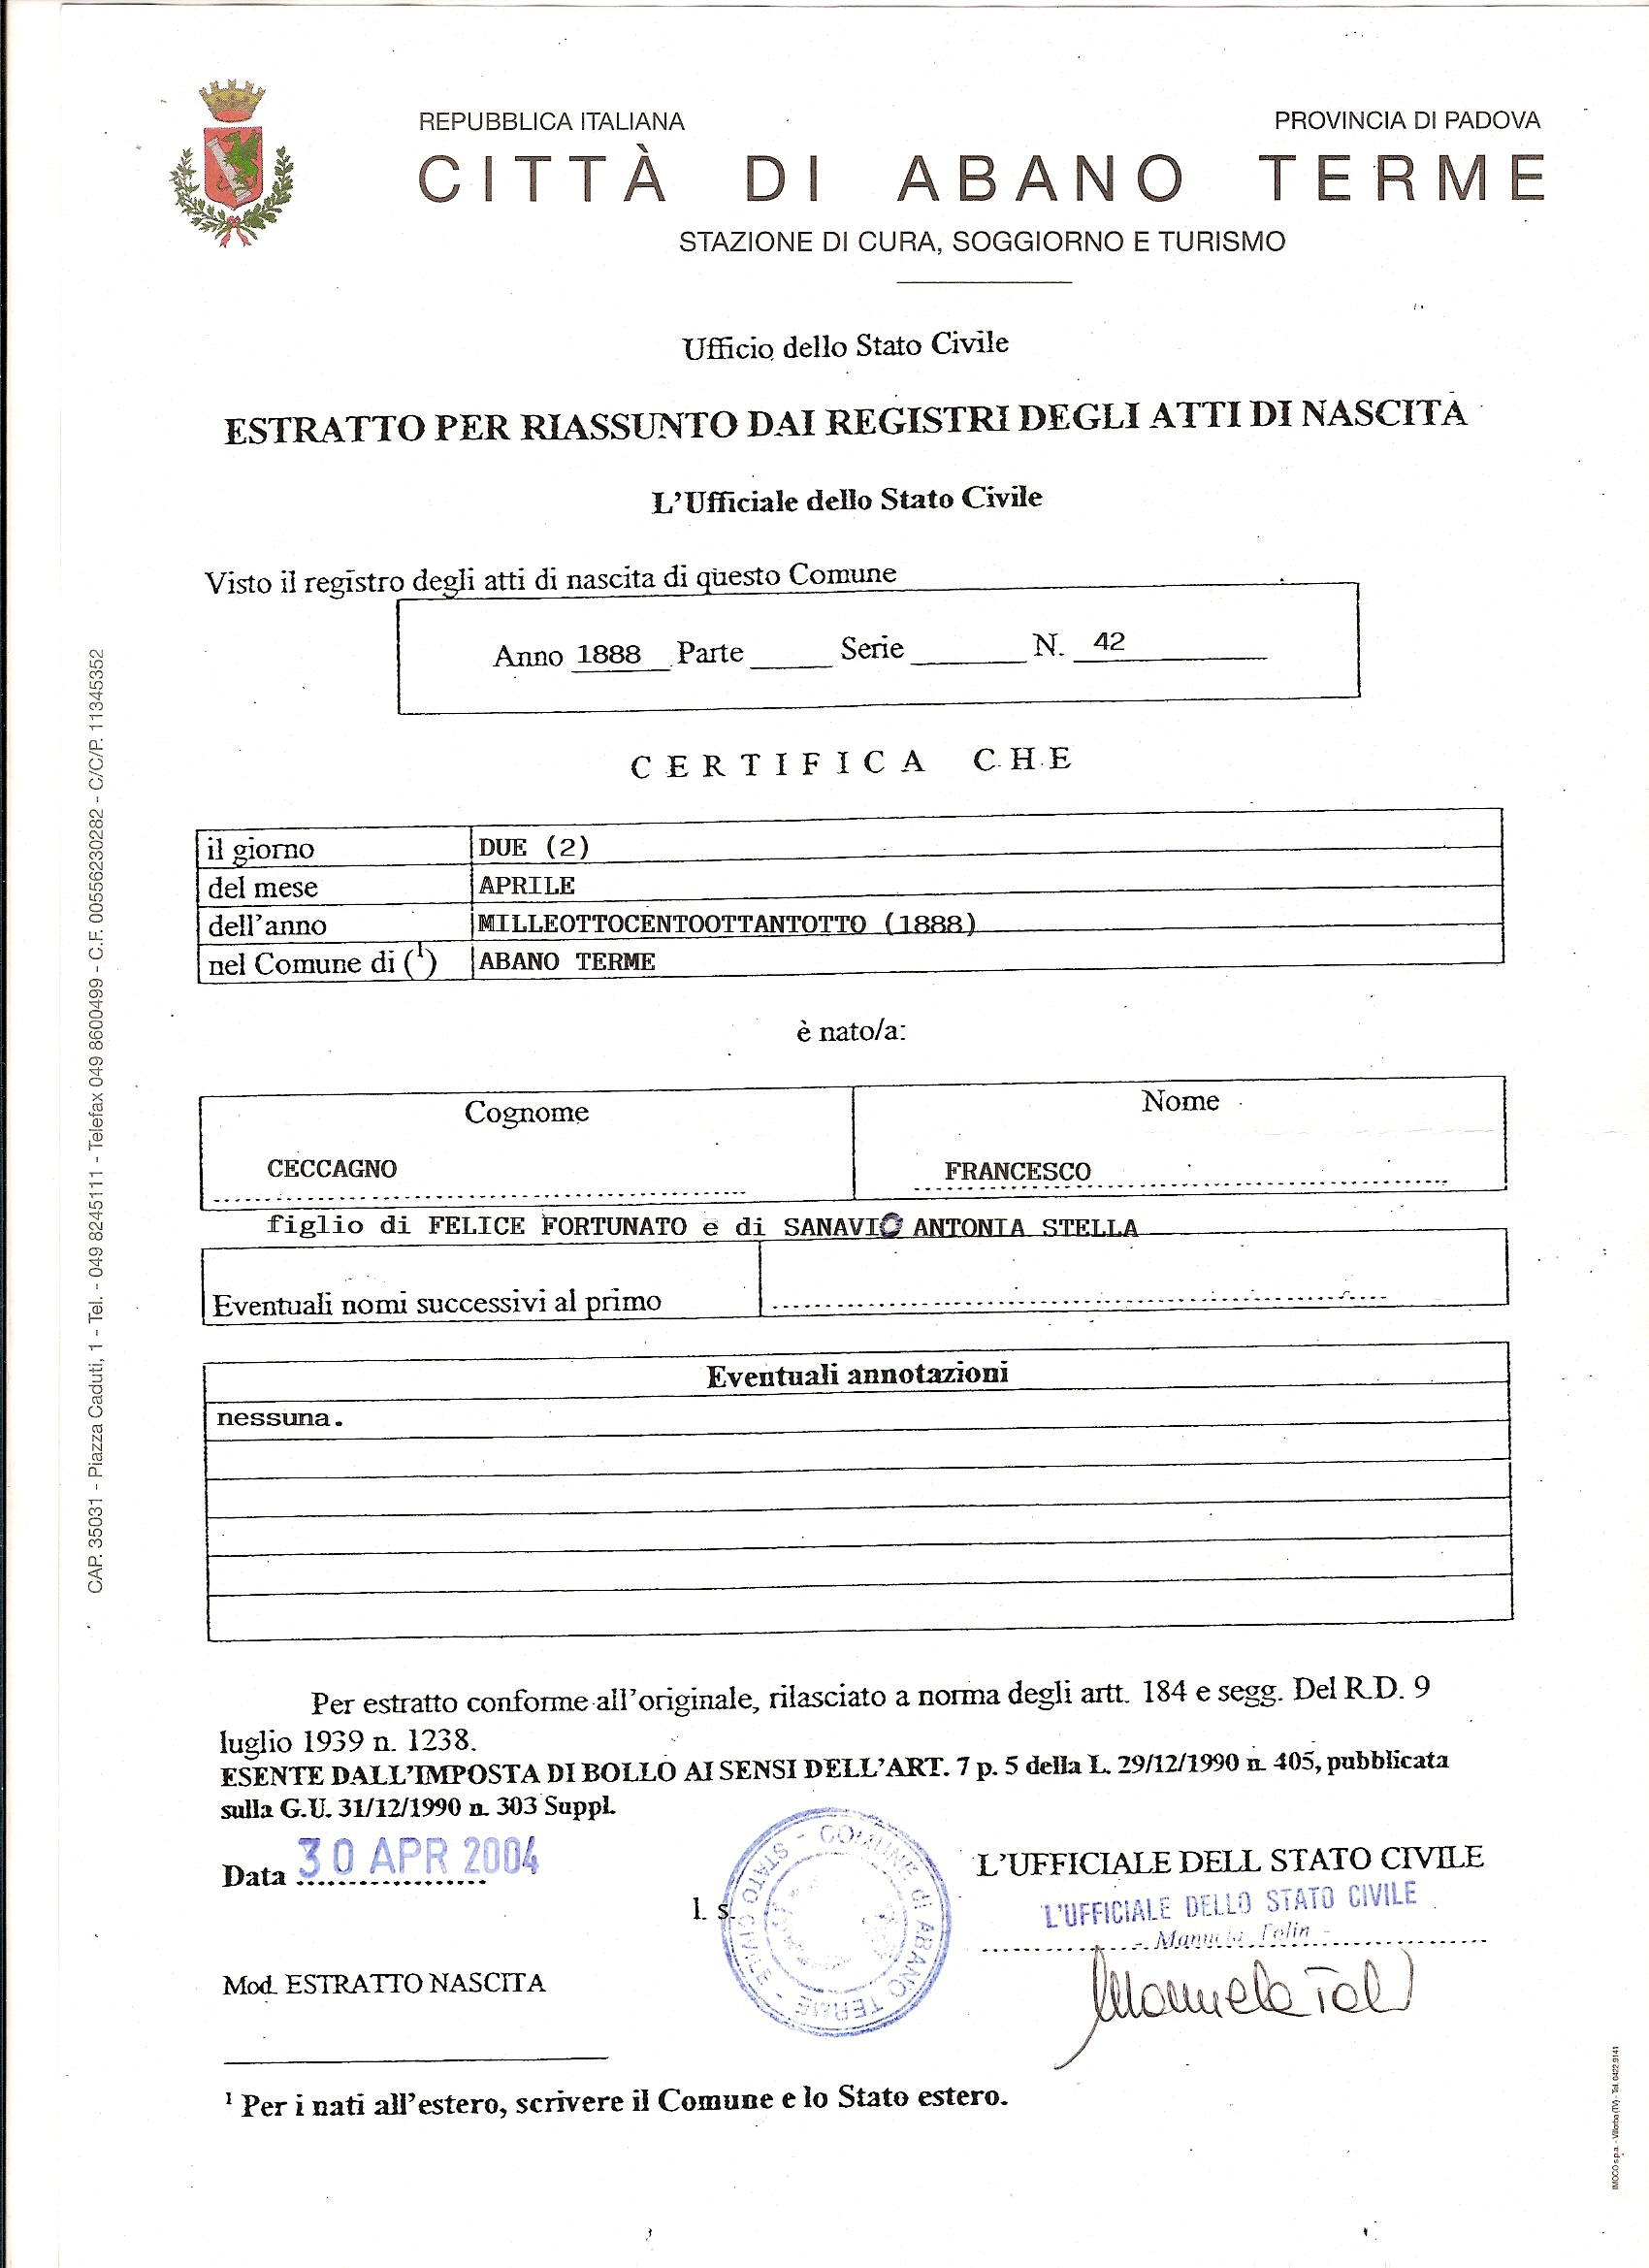
\includegraphics[height=0.35\textheight]{../img/08-francesco.png}\label{fig:08-francesco}
  \\ \\
  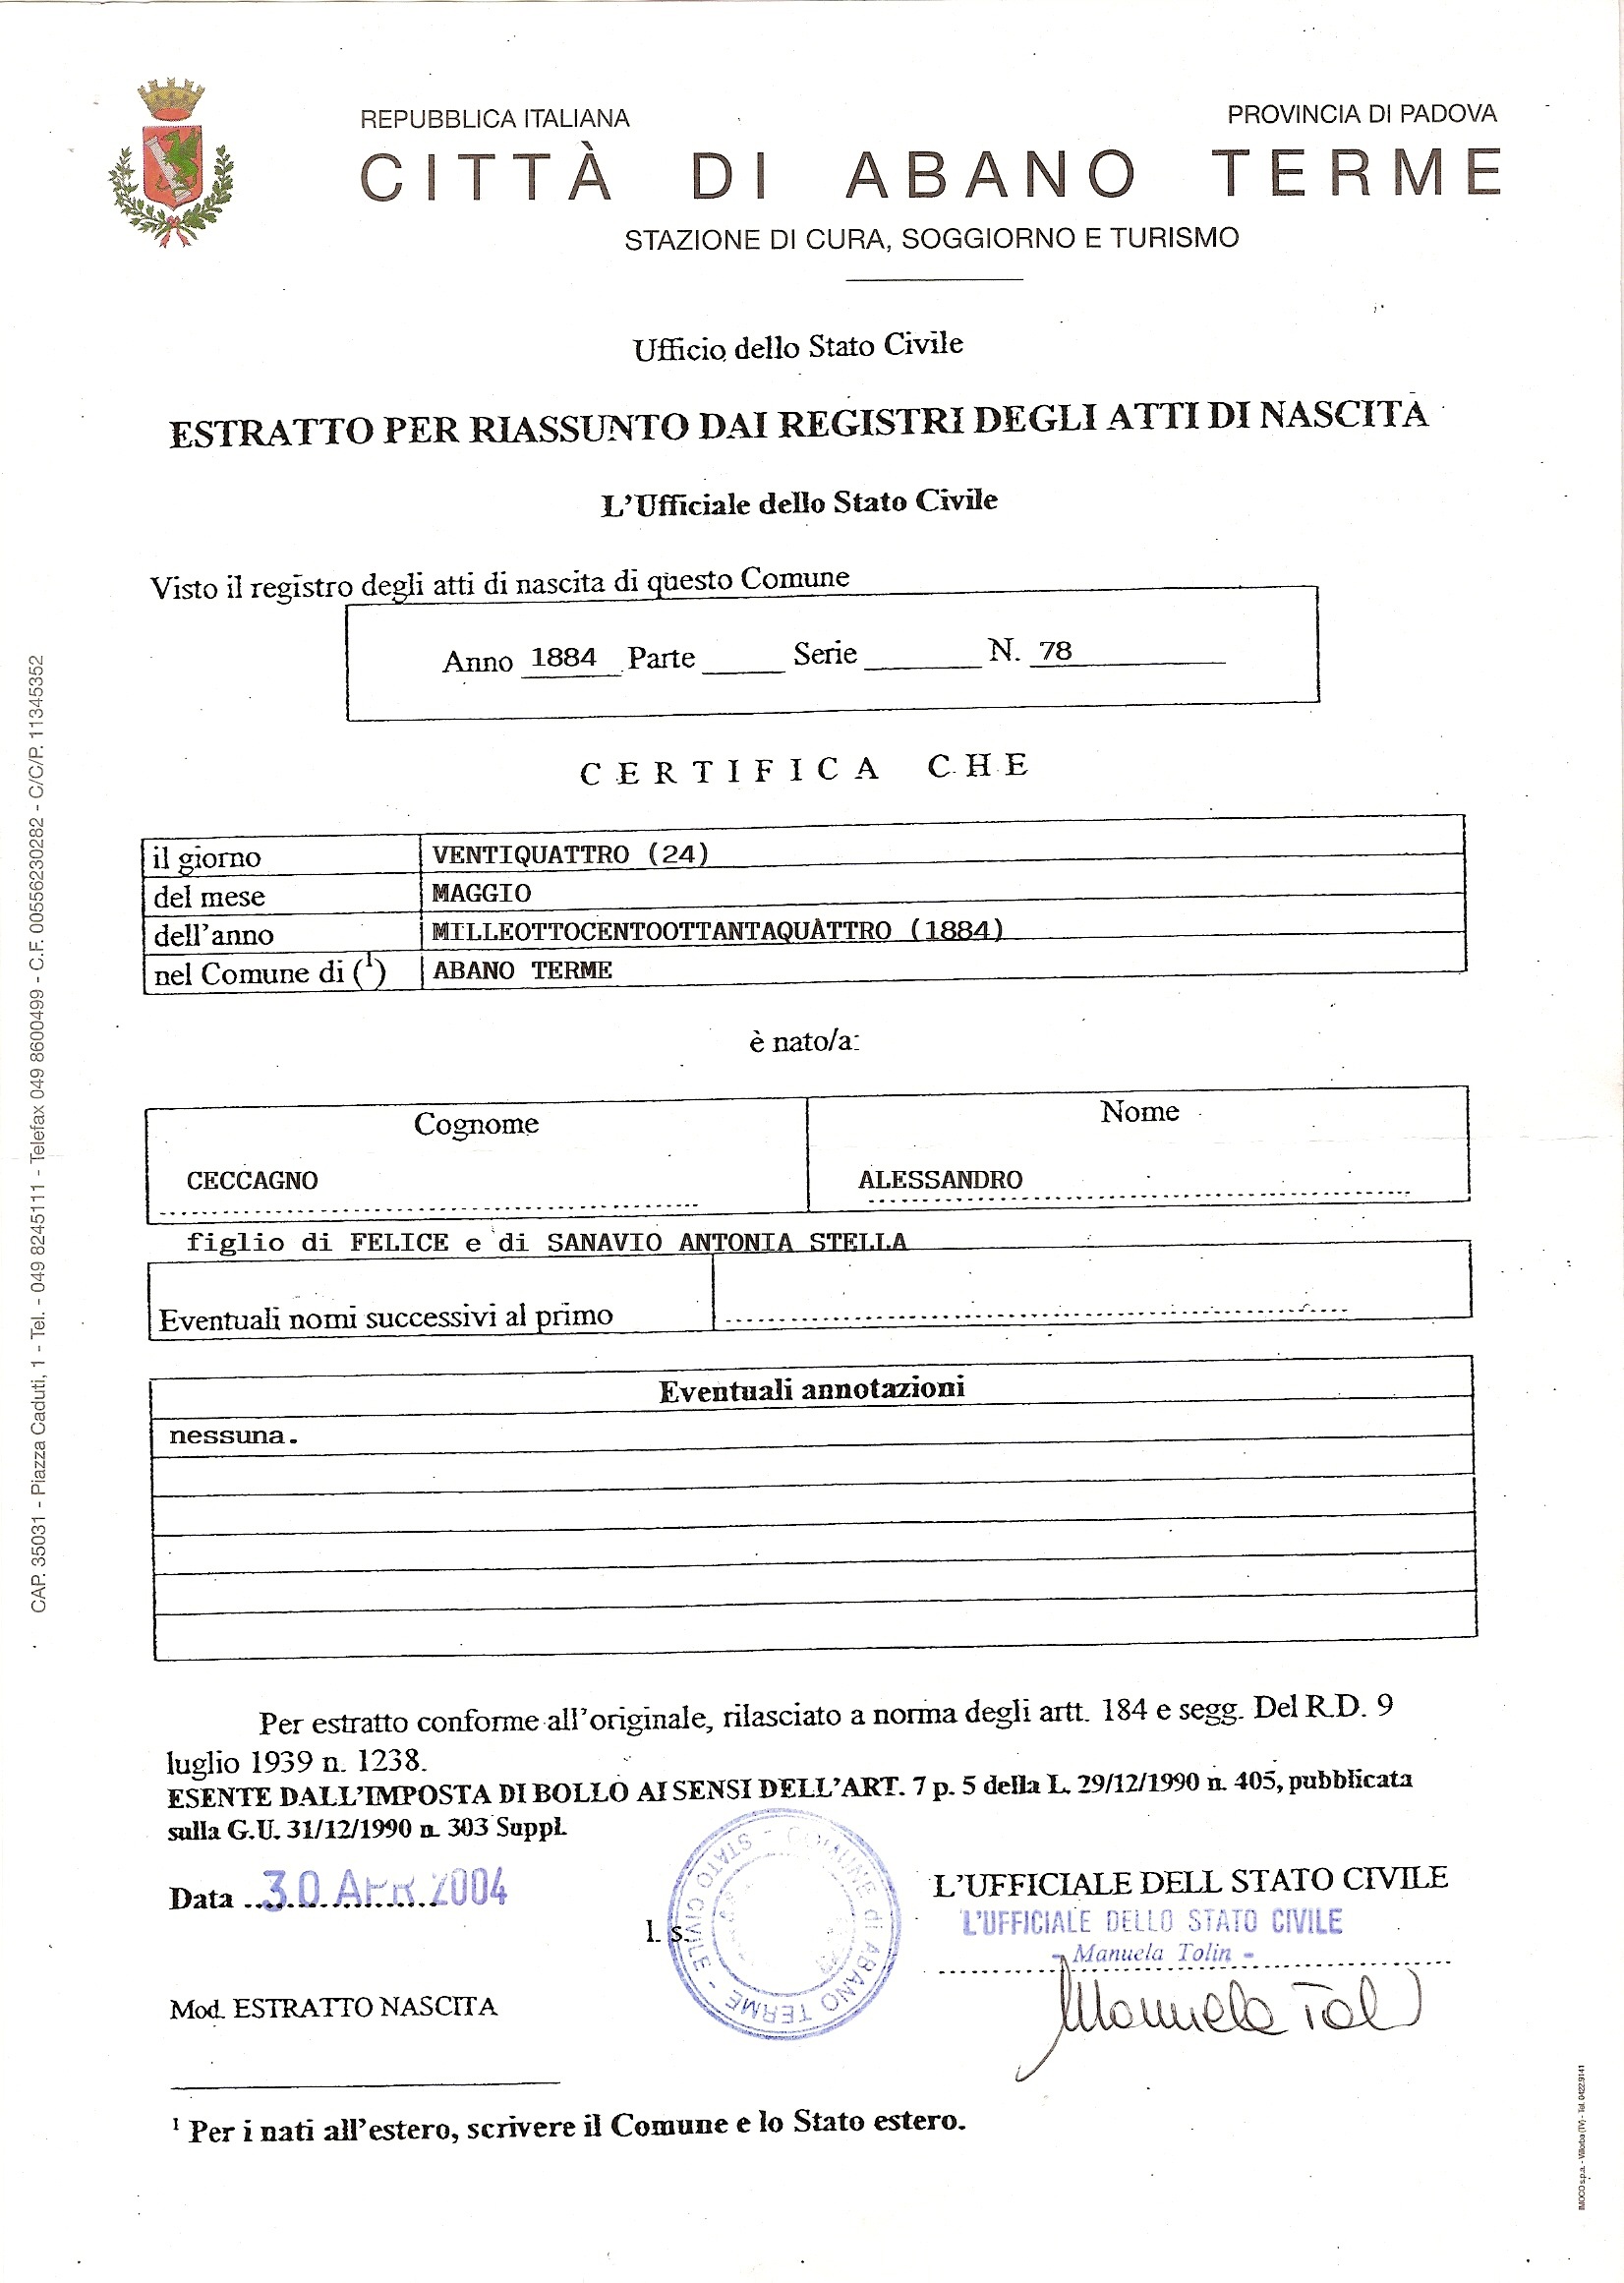
\includegraphics[height=0.35\textheight]{../img/09-alessandro.png}\label{fig:09-alessandro}
  &
\end{tabular}

\chapter*{Preambolo}

\section*{Ricardo}

\textbf{Un giorno ricevo una telefonata da mio cugino Nèreo, dice che sua figlia Antonella ha ricevuto, in data 11-05-2001, una e-mail dal Brasile. Lo scrivente era un certo Ricardo Cecagno (una sola C \emph{por erro do cartorio}, stava scritto). Fra l’altro diceva che gli \emph{gostava muito descobrir} che, in Italia, esistessero ancora dei Ceccagno (come vedremo, non aveva tutti i torti) e che gli sarebbe piaciuto corrispondere con qualcuno, per conoscere il luogo d’origine dei suoi \emph{antapassados}, in particolare di suo bisnonno Alexandre e del padre di questi, Felice.}

Dissi a Nereo di inviarmi una copia dell’e-mail, che ancora gelosamente conservo. Intanto cercai di studiare un poco il portoghese, per imparare quel tanto che mi permetesse di affrontare un minimo di conversazione con il Ricardo, anche perché, aveva precisato, di non sapere bene ne l’inglese e neppure l’italiano.

Finalmente decisi di telefonargli, senza sapere che mi attendeva una stupefacente sorpresa. 
Ci fu una certa difficoltà nel collegarmi, intanto ripassavo mentalmente le solite frasi di presentazione. “Alò? Eu sou Rolando …..hei recebido…”, sudavo cercando di capire quanto mi diceva lui, in stretto portoghese. Nella foga della conversazione, ad un certo punto e senza accorgermi, mi misi a parlare in italiano. Ricardo rimase silenzioso. Pensando ad una caduta della linea, ripetei: “pronto”. E lui : “no’ gò capìo gnente!” “Ma alora te parli come mì”, ghe digo ! Il resto della conversazione fu più facile.\newline
Mi spiegò che suo nonno Agostinho, 80 anni, lavora ancora, come “ferreiro”, con suo padre Eduardo e lo zio Plinio “el mais velho”, che lavorano “falando” sempre em dialetto. Pensai alla loro costanza nel tramandare, di padre in figlio, la parlata veneta. Dico veneta perché il loro è un misto di padovano-trevigiano con una certa prevalenza di quest’ultimo, che io ben conosco avendo trascorso parte della mia infanzia sulle rive del Piave dai Sartor, parenti di mia madre.

I mesi successivi ci scambiammo notizie e fotografie. Io cercai di indagare presso Comuni, Chiese e Cimiteri , alla ricerca dei Ceccagno oltre a quelli che conosco (e sono quasi tutti), per scoprire qualche legame con quelli brasiliani. Niente! La ricerca fruttò soltanto un notevole incremento del mio albero genealogico. Trovai, e trovo, uno zoccolo duro da superare : la disponibilità dei Parroci a  collaborare, ossia consultare o far consultare gli archivi. E’ molto strana questa mancanza o forse sono io che me la prendo troppo “calda”.

Un giorno, Ricardo, mi invia la copia di un elenco estratto dal registro degli sbarchi di immigrati italiani, nel porto di Rio Grande do Sul, L’aveva reperito nell’archivio Historico di quella città. Frà gli sbarcati c’erano anche : “ Ceccano Felice 44 anos e Antònia 37 com Dionisio 8 anos, Alessandre 6 anos e Francesco 2 anos, chegaram em 1891 SA71 folha 193 n 8667-71”. L’arrivo del bastimento doveva essere avvenuto il 26/02/1891 perchè questa data è indicata per una persona col n°8652, cioè poco prima di quello di Felice. Questo ci permise di ottenere, per induzione, quanto meno l’anno di nascita dei componenti la famiglia Dato molto utile da indicare ai Comuni o ai parroci per le ricerche. Nell’elenco dei nomi c’era anche una Veneranda Ceccagno sposata con Angelo Savario. A tal proposito ricordo che, durante una conversazione telefonica, Eduardo mi disse che, quando ero piccolo,  c’era una vecchia “tia”che ogni tanto li veniva a trovare e che proveniva da Lagoa Vermelha. Era forse Veneranda ? 

A seguito di contatti col signor Mignoni, Prefeito di Protasio Alves, che era stato il primo domicilio dei Ceccagno di Felice, ebbi la segnalazione che altri Ceccagno si trovavano a Rio Claro (S. Paolo).\newline
Con le notizie ottenute, nonostante la difficoltà di corrispondere con quelli di Rio Claro, ho redatto una bozza del loro albero genealogico. Il capostipite si chiama Lodovico. Da una lista telefonica trovai anche dei Cecanho. Mi spiegarono che ciò può essere accaduto in seguito all’obbligo di brasilianizzare i nomi da parte del governo di Getulio Vargas negli anni ’40, quando egli si schierò con gli Alleati durante il 2° conflitto mondiale. Un po’ come fece, in Italia, Mussolini con gli istriani e gli ebrei.\newline
L’arrivo, in Brasile, dei  Ceccagno di Rio Claro, è precedente (1888-1889) a quello di Felice. Quindi si può ipotizzare che ci sia stata, fra di loro, una “chiamata”. Anche se sapiamo che in quegli anni fu divulgato, nell’Italia del Nord, un bando del Governo Brasiliano, che cercava manodopera, soprattutto agricoltori, per colonizzare le terre incolte. 

Ho cercato di immaginarmi l’odissea di Felice e famiglia,. con la partenza da Padova per raggiungere Genova, parte in carretto-stop, e parte in treno. Era inverno e c’era la neve. Poi il viaggio in nave, classe economica, 30-40 giorni di navigazione (come diceva la canzone). Qualcuno durante la traversata, nasceva (ho incontrato nell’elenco una bimba di 0 anni ) e qualche altro moriva. Questi, dopo una sommaria funzione religiosa, veniva calato in mare.  

Chissà come, e con che cosa, avranno raggiunto: prima Porto Alegre (650 km) poi Caxias (125 km), dove c’era un centro di raccolta per gli emigranti. Qui, venivano assegnati a credito, mezzo certamente utilizzato da Felice, degli appezzamenti di terreno. Anche di 150.000 mq.

Come detto, lo Stato di Rio Grande do Sul, era interessato a colonizzare quelle terre. Tale opportunità veniva pubblicizzata, attravverso le ambasciate, negli Stati europei.\newline
Le terre più facili da ottenere e meno costose, erano quelle selvagge, boscose e collinari, quindi sassose; insomma: la parte coltivabile doveva essere rubata alla natura. Per fare questo ci volevano: grande volontà, braccia forti e…   tanta fame. Queste qualità erano, sicuramente, l’unico patrimonio in possesso di chi partiva dal Veneto in quegli anni. Il miraggio dell’emigrante era quello di diventare “padrone” del suo pezzo di terra.\newline
Ricordo quanto succedeva dalle mie parti negli anni ’30, e da quello che mi raccontava mio nonno Filippo per gli anni precedenti. Le terre erano, in gran parte, in mano a pochi proprietari. Al contadino (allora era quasi l’unico mestiere nel Veneto) non restava altro che “andare a opara” e fare, cristianamente, dei figli. Andare a opara, voleva dire attendere la chiamata per andare lavorare a ore la terra altrui. Il lavoro era precario sia d’estate e ancor più, d’inverno. Se poi pioveva...\newline
La retribuzione era: : poca in schei e il resto in natura. Ecco perchè, ad esempio, le braghette dei ragazzini venivano confezionate col “cavallo” all’altezza del ginocchio, in modo che alla crescita del ragazzo, si alzava automaticamente, accorciando le “tirache” (bretelle).

\section*{Nonno Filippo}

Nonno Filippo fu un mito per me. Ho trascorso molto tempo della mia infanzia con lui.\newline
Dieci figli, a ciascuno dei maschi procurò una attività commerciale. Così come  fece anche Agostinho con i suoi 11 figli e Pedro Antonio per i suoi 8. Che sia un vizio-virtù dei Ceccagno?  
Filippo in gioventù faceva “el scarparo”, come Felice, ma gli piaceva fare il contadino. Per questo aveva acquistato vari terreni che coltivava o faceva coltivare. Dopo avere fatto il calzolaio, aveva acquistato un forno e un’osteria, dove si ballava al suono di un’organetto a tamburo. Veniva caricato  a molla e si metteva in moto con la monetina. La sala dedicaa al ballo, era dotata di due porte, una per l’entrata ed una per l’uscita. Le persone che entravano, pagavano e, dopo un certo numero di balli, erano costretti ad uscire accompagnati da una corda che, fissata presso la porta d’uscita, veniva azionata  da un’addetto. Chi voleva rientrare, ripagava il biglietto.

Installò anche, all’aperto, un cinema muto. Erano gli anni della Prima Guerra Mondiale, alla quale tutti e cinque i figli maschi, parteciparono.

Con mia nonna Cecilia non aveva molto tempo per dialogare. C’è un aneddoto che può spiegare come fossero stringati i loro dialoghi.\newline
Mio nonno era appassionato degli animali da stalla. Aveva una “musseta” con la croce bianca sulla schiena. La leggenda dice, che anche quella della fuga in Egitto della Sacra Famiglia, avesse tale simbolo sulla schiena. Inoltre, in stalla, teneva un altro somarello. Ma la regina della compagnia era : la CAVALLA!.\newline
La impiegava, attaccata alla  “barachina”, un elegante cocchio, quando si recava, soprattutto, in piazza a incontrare gli amici per una chiaccherata davanti a “un’ombra” di bianco o nero. Ma anche per “stimarsi”, farsi vedere.\newline
Un giorno andò alle “Fiere di Battaglia Terme” che, in quei tempi, erano una importante manifestazione annuale, dove si offrivano o  si acquistavano : animali domestici, sementi, attrezzi agricoli ecc.

Vide una cavallina stupenda, giovane, vispa, forse fin troppo.Tornò a casa e lo disse alla nonna : “ Femena, a gò visto na’ cavaina che…”, Non fece in tempo a concludere la frase che la nonna, senza guardarlo, l’anticipò con : “Comprala!”. E lui la comprò.

Alla domenica successiva, verso le 11, quando la gente, finita la messa, si riuniva in piazza, lui attaccò la cavallina alla “baracchina” e si avviò. La cavalla aveva un incedere altero, la testa protesa leggermente all’indietro richiamata dalle redini unite al morso. Una leggera bava bianca intorno alla bocca. Insomma il nonno pregustava una “stimata” mica da ridere!\newline
Arrivato in piazza,  la gente : “Varda ciò, Fiipo”.\newline
Lui tentò di rallentare e fermare l’animale che, invece, si diede a scalciare, innalberarsi e nitrire. Dovettero intervenire gli amici per amansirlo.\newline
Tornò a casa; alla nonna, indaffarata con le pentole, intorno al focolare, disse soltanto : “Femena, pensa cossa me gà comb..” , anche qui il suo dire fu troncato da un perentorio : “Vendela!”.

Il nonno mi raccontò anche un altro aneddoto comico, sulla fiera.\newline
C’era un contadino che , ogni anno, si ostinava a proporre in vendita un suo cavallo. Si sa che i compratori, non fidandosi dell’età dichiarata dal venditore,  con le mani alzavano il labbro superiore del cavallo scoprendo la dentatura. Si dice che, dalla dentatura, si possa dedurre l’età dell’animale. Ora, quando il cavallo vedeva avvicinarsi qualcuno che, parlando, avesse le mani in movimento, lui rovesciava, nitrendo, il labbro superiore mostrando la dentatura, anticipando le intenzioni anche di chi non le aveva per niente.
 
Spesso andavo a trovarlo in campagna, nel suo casotto fatto di canne di granoturco, dove teneva, fra le altre cose, alcuni vecchi giornali ingialliti che mi leggeva facendomi la traduzione simultanea in dialetto veneto, poichè era la sola lingua che, allora, conoscevo.\newline
Durante la settimana Santa, le campane rimanevano mute.Il segnale del “mezzogiorno” veniva dato da noi ragazzi, azionando le “racoete” (raganelle). Erano degli strumenti ottenuti da un blocchetto di legno di sezione quadrata. Esso veniva scaricato riducendo a una lamina tre lati. Uno di questi veniva assotigliato e reso libero, sarebbe stato quello che avrebbe prodotto il suono. Sui due lati contrapposti, veniva montata una ruota dentata bloccata sul suo perno, sul quale era fissata un manovella.\newline
Il nonno aveva una incredibile cognizione del trascorrere del tempo. In quella settimana noi lo raggiungevamo nei campi. Lui ad un certo punto ci dava il segnale  di azionare le “racoete” : era mezzogiorno.  In quel momento scattavano le “racoete” dei ragazzi di tutto il paese.
 
Era contro ogni forma di oppressione, amava la libertà per se e per gli altri, insomma : alla Garibaldi. E’questo un sentimento  che mi ha inculcato. Un esempio? 

Un giorno del 1935 mi trovavo con lui, mentre in piazza c’era una manifestazione fascista. In quei tempi veniva installato un’altoparlante collegato alla radio delle scuole. Ad un tratto ci arriva una voce, era quella di Mussolini. Mi guardò e mi disse :\textbf{``Quel che lo scolta, l’è on popolo sucòn, te vedarè dove el ne portarà``}. Eravamo nel 1935. Avevo 8 anni, questa profetica frase mi rimase impressa. Il culto della personalità è sempre pericoloso, e nonno Filippo, purtroppo, avrebbe avuto ragione.\newline
Infatti vi fu la guerra con l’Abissinia, seguita da quella di Spagna e, infine, la drammatica seconda Guerra Mondiale. 

Era un valente cacciatore, ricordo che si accompagnava con Reno, il suo fedele cane. Come me, amava gli animali.

\begin{figure}[htp]
\centering
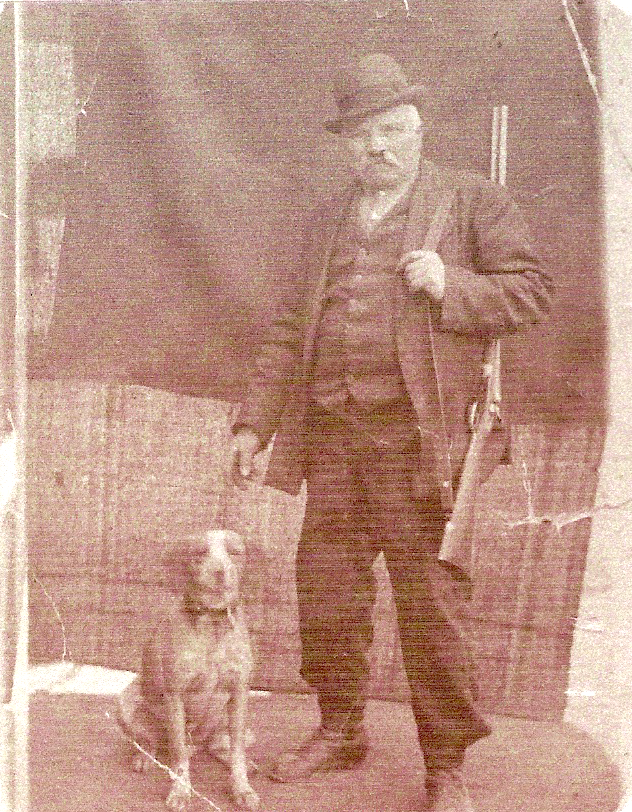
\includegraphics[width=0.3\textwidth]{../img/10-filippo.png}\label{fig:10-filippo.png}
\caption{Filippo con Reno}
\end{figure}

\section*{Gioanin Pulse}

Quando lessi la e-mail di Ricardo, pensai a mio nonno ché mi aveva parlato, sia pure vagamente, di Ceccagno emigrati in Brasile.\newline
Scoprii, in seguito, che una sua sorella, Caterina Ceccagno Sanguin, era emigrata in sud America col marito e sei figli. Uno di questi, Gioanin Sanguin Ceccagno, alias Gioanin Pulse, conosciuto comunemente come Gioanin “bocastorta”, fece ritorno negli anni ’30. Lo conobbi e gli volevo bene. Provavo per lui una grande tenerezza. Tutti pensavano che fosse tornato “pien de schei”, invece dovette adattarsi a fare per mio nonno, il contadino tuttofare. Si accontentava di dormire nella “tesa” (fienile). Mangiava quasi sempre, appartato. Però aveva una sua dignità.\newline
Infatti, alla domenica, si recava in piazza vestito con l’unico abito, di lino bianco, che si era portato dall’America, il cappello di panama, con la tesa destra abbassata alla moda di allora, e il bastone di bambù. La barba intorno alla bocca, gli celava il diffetto fisico che aveva generato il sopranome. Rispetto alle altre persone, reduci dalla Messa grande delle 11, sembrava un damerino. Qualcuno gli proponeva : “Gioanin on’ombra?” E lui, con un’atteggiamento fiero, si concedeva con un : “Ma sì!”

Dopo molti anni, lo incontrai nella “casa di ricovero” peri vecchi. Io allora vivevo a Milano. Mi chiese di procurargli un canocchiale per osservare il cielo stellato. Sapevo che era un’appassionato di astronomia. Mi rimane il rammarico di non essere riuscito ad esaudire il suo desiderio : morì prima. Fu assistito da quell’angelo custode che è la nostra cugina Carmen Gareggio-Ceccagno, che tutti amiamo per la sua dedizione al prossimo.\newline
Nessuno sapeva perché mio nonno l’avesse accolto con sé. Soltanto con le ricerche per la stesura del mio albero genealogico, più di 40 anni dopo, scoprii che era suo nipote. Entrambi erano già deceduti portanto con sè il segreto del loro rapporto di parentela.

\section*{Felice Ceccagno e famiglia verso il Brasile}

Ma torniamo all’odissea di Felice. Come diceva Afonso, “el gera partio da Genoa co la neve e l’è rivà col caldo e co la ùa e le angurie. I ghe nà  comprà una , mesa i la gà magnà subito e mesa quando i ze rivà a Caxias (piuttosto inverosimile).\newline
Mi piace pensare che sia partito dal porto di Rio Grande e arrivato a Caxias, a tappe.\newline
Già allora le terre più lavorabili erano accaparrate da spagnoli, portoghesi e dai più “furbi”. I nostri avrebbero dovuto accontentarsi di pezzi di “mato” e rocce comprese, posto in zone collinose.

Le mie ricerche sulle “raise” di Felice durarono fino al 30 aprile del 2004 quando, dal Comune di Abano Terme, mi pervenirono i certificati di nascita di Giosuè Dionisio 1882, Alessandro 1884, Francesco Isidoro 1888, Maria 1879, Filomena 1885, Antonio 1887. Questi ultimi tre deceduti, probabilmente, prima della partenza. I Ceccagno del Brasile avevano sempre creduto che i figli di Felice fossero solamente tre.\newline
Continuerò la mia ricerca per trovare l’aggancio fra il mio ramo e quello di Felice.\newline
Ricardo fu felicissimo della scoperta, perchè poteva finalmente avviare le pratiche per ottenere la doppia nazionalità.\newline
Intanto lui mi aveva messo in contatto con la disponibile e premurosa Janete del ramo di Pedro Antonio , e con suo marito Gelson, col quale ebbi un  incontro, a metà 2004, a Milano. Era venuto in Europa per lavoro.\newline
Timori su come intenderci non esistevano. Ogni telefonata, con Agostinho, Eduardo, Paulo Luiz e sua moglie Ebe, era un torrente di parlata in veneto.\newline
E’ con queste premesse, qualche foto di loro e qualche immagine dei luoghi, che io e Virgina, l’11 agosto 2004, decidemmo di  partire, anche a seguito di una lettera di Ricardo. Infatti, fra l’altro, mi comunicava che il suo nonno Agostinho avrebbe festeggiato il suo 60° di matrimonio. “Perché non venite, sarebbe un grande regalo per lui e mia nonna Ofelia”.\newline
Per un momento pensai che sarebbe stato un bel colpo di testa, visti i miei 77 anni e qualche acciacco. Dopo due giorni decidemmo di accettare l’invito.

\chapter{Diario del viaggio in Brasile}

\section*{11 agosto 2004}

All’aeroporto di Malpensa ci accompagna mio figlio Claudio. Fa caldo, allora prendiamo una birra e un coca-cola, al banco. Costo \euro 8,50. Dico questo perché, come vedremo in seguito, in Brasile con quella cifra si pranza in tre persone.

Timori? Ansia per il viaggio in aereo? Non molta, anche se un pensiero al….testamento, l’abbiamo fatto.
Ci aspettavano 13.000 km e 18 ore di volo, con un trasbordo a S. Paolo.
Si parte alle 22. Ci avevano dato dei consigli : alzatevi, camminate spesso, dormite, ecc. Dice : per chi non ci riesce ci sono i film,  che vengono proiettati su un piccolo schermo posizionato sullo schienale della fila di fronte. Risultato : la cuffia non regge, il telecomando non funziona o non lo sappiamo usare.

Virginia dorme spesso, mentre io mi limito a guardare le informazioni sullo schermo centrale : velocità media 9.500 km/h in 11.5h = 800 km/h, temperatura esterna –45°C. Penso se non dovesse funzionare il condizionamento, o peggio, la pressurizzazione. Sul monitor appare in continuazione la posizione del nostro aereo rispetto al percorso.

I posti sono comodi. Le file sono 3, quella centrale è a 4 posti, le laterali a 3.Noi siamo su quella di sinistra. Il posto vicino al finestrino è occupato da un signore di colore, piuttosto giovane. E’ poco interessato al panorama, come, invece, lo saremmo noi. Del resto, i nostri posti, sono situati all’altezza di un’ala, per cui si vede poco. Il nostro compagno di viaggio è silenzioso, solo qualche cenno di sorriso. In seguito faremo una fugace conoscenza. E’ di Pernambuco, quindi, al cambio di S. Paolo, prenderà un volo diretto a Natal, che si trova nel nord del Brasile. E’ una località turistica, molto nota e apprezzata dagli italiani. Ne abbiamo conferma da un colloquio fra lui e un gruppo di turisti veneti, uno dei quali parla bene il portoghese. Il pernambuchese, infine ci risulterà simpatico.

Ora fa buio, si notano i faretti lampeggianti sull’ala dell’aereo. Viaggeremo al buio fino a circa 1000 km da S.Paolo. Finalmente dal finestrino si vede il mare e, all’orizzonte, la costa che però risulterà sempre là per molto tempo. Ci vorrà ancora quasi un’ora prima che si avvicini. Sono circa le 2 del 12 agosto, le 7 in Italia. Fra un’ora e mezza atterreremo a S. Paolo L’aereo farà prima un lungo giro verso nord, all’esterno della città.
Qualche sobbalzo, poi, finalmente, siamo sopra la terraferma. Mi alzo, sotto di noi si vedono delle catene montagnose.
Mi viene da pensare : in caso di atterraggio, diciamo, forzato, sarebbe preferibile avere sotto, il mare o la terra? Vedendo i picchi di quelle montagne, decisamente, il mare, contrariamente a quello che avevo pensato prima, quando vi eravamo sopra.
Finalmente rivediamo il mare, il rumore dei motori sale, vengono alzati gli alettoni frenanti, l’aereo scende, ora, velocemente.
Ecco S. Paolo, la sua estensione è impressionante, i grattacieli si avvicinano, ancora qualche sobbalzo. Ci siamo!
Virginia, che mi teneva stretta la mano (o forse ero io), ha un sospiro di sollievo. Una strana pace ci pervade. Non ci eravamo accorti di quanta fosse l’ansietà che ci attanagliava. 
Un momento, c’è ancora da affrontare il tratto da S.Paolo a Porto Alegre, che è di 1500 km., una bazzecola : un’ora e mezza di volo.

Osserviamo i passeggeri che devono ritirare i bagagli. Meno male che noi abbiamo convenzinato che ci vengano recapitati direttamente a Porto Alegre. Almeno, così pensiamo.

Virginia, pensando al prossimo volo, mi dice : “senti, come la và la và”. Ci è subentrata una certa, chiamiamola, rassegnazione. Siamo stanchi di pensarci e, di conseguenza, di angosciarci. 

Abbiamo, purtroppo, circa 3 ore di attesa che, però, fra controllo dei documenti evisite ai negozi,  trascorrono abbastanza velocemente. 

L’aeroporto è enorme, c’è da camminare parecchio per raggiungere la “porta” d’imbarco. I negozi sono dotatissimi, osserva Virginia, salvo i free-shop, piuttosto deludenti. Arrivati, ci sediamo accanto a due signore che mi sembrano molto disponibili a dialogare. Mi rivolgo verso loro in uno stentatissimo portoghese. Mi rispondono felici in italiano ! Brutto segno, difficilmente impareremo il portoghese nel mesetto che trascorreremo da queste parti. E non sappiamo cosa ci aspetta!

Si parte per Porto Alegre alle 8,45. A bordo ci viene servita la colazione : cappuccino con brioches, poi burro, marmellata, prosciutto, formaggio, frutta, caffè (poco degno di questo nome per l’intenditrice Virginia) latte e tè. Alla faccia!
Questa volta la nostra posizione in aereo è tale da permetterci di ammirare il paesaggio sottostante. Ne siamo contentissimi!

Ci avviciniamo a Porto Alegre, mi sembra di scorgere il rio Guaìpa che si getta nella enorme Lagoa dos Patos. Ricordo di avere letto che Garibaldi compì qualche azione importante, da queste parti, quando combattè, negli anni 1839/41 agli ordini di Bento Gonçalves, nella guerra per l’indipendenza dello Stato di Rio Grande do Sul.

Scendiamo dall’aereo alle 10, in perfetto orario. Ora l’emozione, che ci prende, è un’altra : quella dell’incontro con Ricardo e Janete.
Incolonnati e guidati da una transenna, seguiamo il percorso che ci conduce ai controlli. Dichiarazioni varie per la dogana e la polizia di Stato. Quanta moneta : \euro 500 a persona. OK.

\section{Dunga}

Attendiamo, davanti al tapìs-roulant, il nostro bagaglio. Arrivano tutti, meno il nostro. La sala si svuota,momento di panico. Forse abbiamo sbagliato postazione? No! Ciconferma una guardia interpellata. I nostri bagagli non sono arrivati. Che si fa? Pensiamo che, fortunatamente, i bagagli sono stati sigillati, alla partenza, dall’adetto dell’agenzia presso la quale sono stati assicurati (credo per \euro 500). Misera consolazione!

Ci ivolgiamo, col nostro improbabile portoghese, alla polizia interna. Non ci comprendiamo.
Penso a Janete e Ricardo che ci attendono, loro ci potrebbero aiutare. Lo diciamo al poliziotto, ci dice di chiamarli, anche perché, si è reso conto, il dialogo fra noi si è reso imbarazzante. 
All’uscita un altro poliziotto mi blocca. “Se uno di noi esce, non può più rientrare”, mi dice. “Inoltre, prevenendo la mia richiesta, nessun estraneo può entrare senza regolare permesso”. E io come faccio avvisarli? Cerco di spiegarmi, imploro. Niente da fare. 

Finalmente una botta di fortuna. C’è un signore che sta per uscire e che si era fermato ad ascoltare. Cerca di intervenire in mio favore. Sarà un italiano, mi dico. Lo guardo e lo  riconosco. Sbotto tutto d’un fiato : “Lei giocava nella Fiorentina, tirava le punizioni da dio, era un duro e mi piaceva molto, anche se io sono interista”. E aggiungo : “Lei è Dunga!” Resta piacevolmente sorpreso. Mi sorride e : “Sì, sono io” Mi stringe la mano. La guardia è sorpresa. 
Lui mi invita, in perfetto italiano, a stendere la denuncia, ed essere fiducioso.: “Qui non si ruba”, aggiunge. Poi si rivolge al poliziotto a guardia dell’uscita, gli dice qualcosa. Poi, dopo avermi abbracciato, mi dice : “Domani alle 10 le valigie saranno a casa tua, ciao”.
Mi rammarico che, a causa del trambusto, non mi sono fatto fare, da Virginia, una foto.
Il risultato, però, è che arrivano Janete e Ricardo.

Si sono incontrati per la prima volta in aeroporto. Anche questa è una conquista dovuta, molto modestamente, alle mie ricerche.
Con loro completiamo la denuncia.

\section{Janete}

All’uscita dall’aeroporto, c’è un signore che ci fa delle foto, mentre un altro regge un cartello con la scritta : “BENVENUTTI A ROLANDO E VIRGINIA” e il tricolore. Abbracciamo tutti.

Janete ha fatto le cose per bene, mi accorgerò,  in seguito, delle sue enormi doti di organizzatrice. Lei non delega nessuno: lei opera in prima persona. Ha ordinato un pulmino da 10 posti : “Par essere comodi”, dice.

Janete è una bella signora, elegante, capelli e occhi scuri e lo sguardo è molto dolce, sembra timida perché parla poco, ma è soltanto e sempre, in attesa di intuire le necessità e i desideri degli ospiti. Splendida !
Ricardo è più alto di quanto pensavo. Molto affettuoso. Finalmente entrambi, dopo tanti contatti epistolari e telefonici ci possiamo, materialmente, incontrare. Fu lui a gettare il seme con la e-mail a Antonella Ceccagno, docentente di cinese all’Università di Bologna, e autrice di notevoli saggi sui rapporti economico-commerciali Cina/Occidente e le problematiche inerenti. Come detto, Antonella è figlia di mio cugino Nereo. 
Da allora sono trascorsi oltre 3 anni, con molta corrispondenza e telefonate.
Ora siamo qui, in Brasile, conoscerò tutti i miei Ceccagno finora visti soltanto in fotografia o immaginati.
Abbracciamo  anche il signor Sibilla titolare del pulmino e motorista (autista).

A proposito del modo di salutarci : ci si abbraccia, i baci sono trè; si parte da sinistra (in Italia da destra). Per noi, le prime volte, ci troviamo in imbarazzo; spesso avvengono scontri fra i nasi, ciò provoca delle risatine. In contemporanea ci si percuote affettuosamente  e reciprocamente, con la mano destra (non so se per i mancini sia il contrario), la schiena.  Col tempo questa forma di saluto ci risulterà spontanea e molto simpatica.

\end{document}
